\documentclass[a4paper,12pt]{article}

% Зачеркивание
\usepackage{cancel}

% Работа с русским языком
\usepackage{cmap}					% Поиск в PDF
\usepackage[T2A]{fontenc}			% Кодировка
\usepackage[utf8]{inputenc}			% Кодировка исходного текста
\usepackage[english,russian]{babel}	% Языки и переносы

%%% Работа с русским языком
% \usepackage[english,russian]{babel}   %% загружает пакет многоязыковой вёрстки
% \usepackage{fontspec}      %% подготавливает загрузку шрифтов Open Type, True Type и др.
% \defaultfontfeatures{Ligatures={TeX},Renderer=Basic}  %% свойства шрифтов по умолчанию
% % \setmainfont[Ligatures={TeX,Historic}]{Times New Roman} %% задаёт основной шрифт документа
% % \setsansfont{Comic Sans MS}                    %% задаёт шрифт без засечек
% % \setmonofont{Courier New}
% % \usepackage{indentfirst}
% % \frenchspacing

 
% Правила переноса
\usepackage{hyphenat}
\hyphenation{ма-те-ма-ти-ка вос-ста-нав-ли-вать}


% Размеры страниц и отступы
\usepackage[a4paper,top=1cm,bottom=2cm,left=2cm,right=1.5cm,marginparwidth=1.75cm]{geometry}

% Дополнительная работа с математикой
\usepackage{amsmath,amsfonts,amssymb,amsthm,mathtools, mathtext, cite, enumerate, float} % Пакеты АМО
\usepackage{icomma} % "Умная" запятая: $0,2$ --- число, $0, 2$ --- перечисление

% Шрифты
\usepackage{euscript}	 % Шрифт Евклид
\usepackage{mathrsfs} % Красивый матшрифт

% Перенос знаков в формулах (по Львовскому)
\newcommand*{\hm}[1]{#1\nobreak\discretionary{}
{\hbox{$\mathsurround=0pt #1$}}{}}

% Работа с картинками
\usepackage{graphicx}  % Для вставки рисунков
\graphicspath{images/}  % Папка с рисунками
\setlength\fboxsep{3pt} % Отступ рамки от рисунка
\setlength\fboxrule{1pt} % Толщина линий рамки
\usepackage{wrapfig} % Обтекание рисунков и таблиц текстом

% Работа с цветами
\usepackage[usenames]{color}
\usepackage{colortbl}

\makeatletter
\renewcommand{\@biblabel}[1]{#1.} % Заменяем библиографию с квадратных скобок на точки
\makeatother

\bibliographystyle{unsrt} % Список источников в порядке упоминания в тексте

% Меняем везде перечисления на цифра.цифра
\renewcommand{\theenumi}{\arabic{enumi}}
\renewcommand{\labelenumi}{\arabic{enumi}}
\renewcommand{\theenumii}{.\arabic{enumii}}
\renewcommand{\labelenumii}{\arabic{enumi}.\arabic{enumii}.}
\renewcommand{\theenumiii}{.\arabic{enumiii}}
\renewcommand{\labelenumiii}{\arabic{enumi}.\arabic{enumii}.\arabic{enumiii}.}


\usepackage{multicol} % Для нескольких уравнений на одной строке

\usepackage[export]{adjustbox} % Для вертикального выравнивания картинки и формулы на одной строке

\newcommand{\expnumber}[2]{{#1}\mathrm{e}{#2}} % Для записи 1e-4

\usepackage{hyperref} % Для цитирования картинок из интернета

\usepackage[nottoc,numbib]{tocbibind} % Список литературы в содержании

% Листинг кода
\usepackage{xcolor}
\usepackage{listings}

\definecolor{mGreen}{rgb}{0,0.6,0}
\definecolor{mGray}{rgb}{0.5,0.5,0.5}
\definecolor{mPurple}{rgb}{0.58,0,0.82}
\definecolor{backgroundColour}{rgb}{0.95,0.95,0.92}

\lstdefinestyle{CStyle}{
    backgroundcolor=\color{backgroundColour},   
    commentstyle=\color{mGreen},
    keywordstyle=\color{magenta},
    numberstyle=\tiny\color{mGray},
    stringstyle=\color{mPurple},
    basicstyle=\footnotesize,
    breakatwhitespace=false,         
    breaklines=true,                 
    captionpos=b,                    
    keepspaces=true,                 
    numbers=left,                    
    numbersep=5pt,                  
    showspaces=false,                
    showstringspaces=false,
    showtabs=false,                  
    tabsize=2,
    language=C
}

\renewcommand{\scriptsize}{\fontsize{14}{14pt}\selectfont}
\usepackage{titlesec}
\titleformat{\section}
{\normalsize\scriptsize\bfseries}
{\thesection}
{1em}{\scriptsize\bfseries}
\titleformat{\subsection}
{\normalsize\scriptsize\bfseries}
{\thesubsection}
{1em}{\scriptsize\bfseries}
\titleformat{\subsubsection}
{\normalsize\scriptsize\bfseries}
{\thesubsubsection}
{1em}{\scriptsize\bfseries}

\title{Неявные по времени численные схемы для расчета многофазных многокомпонентных течений в цифровом керне}
\author{Забегаев Ю.А.}

\begin{document}

%\maketitle
%\newpage

% \begin{titlepage}

% \begin{center}
% Министерство образования и науки Российской Федерации \\
% \vspace{0.5cm}
% Федеральное государственное автономное образовательное учреждение\\
% высшего профессионального образования\\
% «Московский физико-технический институт\\
% (национальный исследовательский университет)»\\
% \vspace{0.5cm}
% Факультет аэрофизики и космических исследований \\
% \vspace{0.5cm}
% Кафедра вычислительной физики \\
% \end{center}

% \vspace{5em}

% \begin{center}
% \Large \textbf{Неявные по времени численные схемы для расчета многофазных многокомпонентных течений в цифровом керне}
% \end{center}

% \vspace{2.5em}

% \begin{center}
% Выпускная квалификационная работа\\
% (бакалаврская работа)
% \end{center}

% \begin{center}
% Направление подготовки 03.03.01 Прикладные математика и физика
% \end{center}

% % \vspace{6em}

% % \begin{flushleft}
% % Заведующий кафедрой \\
% % проф., чл-кор. РАН,
% % д.ф.-м.н. \hrulefill Виноградов Е.А.\\
% % \vspace{1.5em}
% % Научный руководитель \\
% % к.ф.-м.н. \hrulefill Компанец В.О.\\
% % \vspace{1.5em}
% % Рецензент \\
% % к.ф.-м.н. \hrulefill Пойдашев Д.Г.\\
% % \vspace{1.5em}
% % Студент\hrulefill Березутский А.В.
% % \end{flushleft}

% % \vspace{\fill}

% \begin{center}
% Долгопрудный

% \vspace{0.5cm}
% 2020

% \end{center}

% \end{titlepage}

\section*{Аннотация}
Целью данной работы является исследование неявного по времени численного метода моделирования многофазного течения в микромасштабе при помощь гидродинамического метода функционала плотности. На примере трехмерного нелинейного уравнения теплопроводности изучаются подходы к решению нелинейных систем уравнений, возникающих при использовании неявного метода, реализуется вычислительный стенд для сравнения различных подходов в том числе с применением технологии CUDA. Предлагается архитектурное решение на основе библиотек символьной математики для быстрого и эффективного внедрения новых физических моделей жидкостей без изменения кода. Выводится одномерная система гидродинамического метода функционала плотности и предлагается неявная схема для решения. Проводится исследование сеточной сходимости реализованных численных схем.  На примере изучения зависимости шага по времени неявного метода от максимальной среднемассовой скорости в системе показываются преимущества неявной схемы при определенных режимах течения. Использованные численные методы и архитектурные решения будут положены в основу реализации неявного по времени моделирования многофазных течения в трехмерном поровом пространстве.

\newpage

\tableofcontents

\newpage

\section{Введение}
Настоящая работа посвящена исследованию неявного по времени численного метода моделирования многофазного течения в микромасштабе. Под многофазностью подразумевается течение нескольких несмешиваемых флюидов. Под микромасштабом подразумевается такой масштаб, на котором характерный размер границы между флюидами сопоставим с размером задачи. Для корректного описания системы необходимо учитывать геометрию границы и влияние сил поверхностного натяжения между флюидами.
\par
Моделирование многофазного течения на микромасштабах решает много практических задач. Например, разработка процессов добычи углеводородов включает в себя исследование совместного течения воды, газа и нефти в естественной пористой среде. При бурении скважин для изучения берут пробу породы - керн. Компьютерная томография позволяет получить его цифровую 3D-модель. Разрешаемый размер пор в такой модели будет порядка $10^{-6}$ м.  Исследование свойств течения в керне позволяет подобрать оптимальные методы добычи. Моделирование такого течения может быть быстрее и эффективнее, чем лабораторный эксперимент. 
\par
Для построения системы уравнений, описывающих исследуемые течения, используется гидродинамический метод функционала плотности, рассмотренный в \cite{demyanov, kudinov, dhd_spe}. Данный метод описывает жидкости с помощью непрерывных полей. Фронт границы между жидкостями имеет конечную ширину, где параметры жидкостей меняются резко, но остаются непрерывными. По сравнению с классическим гидродинамическим подходом, рассматривающим границу раздела как фронт нулевой толщины, такой подход обладает некоторыми преимуществами. Появляется возможность единообразно описать движение многофазного течения без введения отдельного уравнения движения для поверхности раздела. Не возникают сложности при учете изменения топологии границы раздела - естественным образом можно моделировать слияние и разделение капель. Поскольку моделируются непрерывные функции, можно использовать более простые численные методы, которые недоступны для разрывных уравнений. В данной работе используются симметричные методы аппроксимации производных, которые были бы менее робастными при разрывных решениях. По этой же причине все решения, вид которых нам неизвестен, должны быть гладкими функциями. Все известные функции, которые используются в полученной системе уравнений, считаются непрерывными и непрерывно дифференцируемыми столько раз, сколько требуется. Для краткости в настоящей работе такие функции будем называть \textbf{гладкими аналитическими функциями}. Здесь термин ''аналитические'' употребляется, чтобы подчеркнуть, что они заданы известными формулами.
\par
Система уравнений, описывающая многофазное течение с учетом влияния сил поверхностного натяжения, полученная с помощью метода функционала плотности имеет вид:
\begin{equation} \label{eq:dhd_system_intro}
\begin{cases}
\frac{\partial n_{i}}{\partial t}+\frac{\partial\left(V_{b}n_{i}\right)}{\partial x_{b}}-\frac{\partial}{\partial x_{b}}\left(P_{i j}\frac{\partial\Phi_{j}}{\partial x_{b}}\right)=\vartheta_{i}^{n}(t,x_{a}) 
\\ \\
\frac {\partial\rho V_{a}} {\partial t} + \frac {\partial} {\partial x_{b}} \left( \rho V_{b}V_{a} - \tau_{ab} \right) + n_i \frac{\partial \Phi_i}{\partial x_a}=\vartheta_{a}^{M}(t,x_{a})
\end{cases}
\end{equation}
Для краткости изложения в данной работе будем называть ее \textbf{системой функционала плотности}. Система решается относительно переменных $n_i$ - мольных плотностей и $V_a$ - среднемассовой скорости. Здесь используются стандартные обозначения для индексов, принятые в других работах по методу функционала плотности. Индексы $i, j$ означают номер компоненты, для которой записано уравнение. Индексы $a, b$ означают проекцию вектора на одну из осей прямоугольной декартовой системы координат в пространстве. Смысл всех используемых функций мы поясним, когда рассмотрим систему подробно в главе \ref{dhd}.
Особое внимание в формуле \eqref{eq:dhd_system_intro} нужно уделить химическому потенциалу $\Phi_i$:
\begin{equation} \label{eq:chemical_potential_intro}
\Phi_i := \frac{\partial f}{\partial n_{i}}+\frac{1}{2}\frac{\partial\nu_{jk}}{\partial n_{i}}\frac{\partial n_{j}}{\partial x_{a}}\frac{\partial n_{k}}{\partial x_{a}}-\frac{\partial}{\partial x_{a}}\left(\nu_{ij}\frac{\partial n_{j}}{\partial x_{a}}\right)
\end{equation}
Здесь $f$ - удельная свободная энергия, а $\nu_{ij}$ - матрица поверхностного натяжения. Как видно, в системе используется 4-я производная $n_i$.
\par
Рассмотрим физические процессы, которые описываются системой функционала плотности. В большинстве решаемых задач их можно классифицировать по характерным скоростям:
\begin{itemize}
\item Медленные - перенос массы
\item Быстрые - процессы, связанные с поверхностным натяжением, например перестроение топологии границы между флюидами
\item Очень быстрые - распространение звуковых волн
\end{itemize}

Так как система моделирует сжимаемые жидкости, среди процессов можно выделить распространение звуковых волн. Мы могли бы пренебречь этим эффектом, поскольку он нас не интересует с практической точки зрения. 
Однако явная схема обязана совершать достаточно маленький шаг по времени, который будет описывать самый быстрый процесс в системе. Это ограничение можно получить при исследовании явной схемы на устойчивость. Оно появляется математически из-за старших производных в системе. Как было показано ранее, в ней присутствуют производные до 4 порядка.
\par
Неявный метод интегрирования по времени лишен такого ограничения. Делая неявные шаги, можно сразу переходить от одного равновесного распределения к другому, усредняя процессы распространения звуковых волн. В работах \cite{kudinov, dhd_spe} реализованы численные методы, позволяющие моделировать многофазное течение на микромасштабе с помощью метода функционала плотности. Они используют явный метод интегрирования по времени. В частности, в работе \cite{kudinov} автор ссылается на недостаточные вычислительные мощности для применения неявного метода. 
\par
Вид гладких аналитических функций $f$ и $\nu_{ij}$ в уравнении \eqref{eq:chemical_potential_intro} определяется физической моделью исследуемых жидкостей. В применяемых на практике моделях они имеют сложный вид. Чтобы использовать такую модель, нужно аналитически вычислить их производные по $n_i$. Для применения неявного метода понадобятся еще и вторые производные. Из-за этого внедрение новых физических моделей в программу становится очень трудоемким. В настоящей работе предложен метод автоматизации этого процесса, не замедляющий расчет.
\par
Целью данной работы является исследование подходов к реализации неявного численного метода решения системы функционала плотности. Анализируются преимущества, которые дает неявный метод. Изучаются характерные особенности и трудности, которые могут стать ''бутылочным горлышком'' в его реализации. Предлагаются способы решения таких трудностей. 
\par
Все методы исследовались сначала на упрощенной задаче - скалярном нелинейном уравнении теплопроводности:
\begin{equation} \label{eq:heat_equation_intro}
\frac{\partial u}{\partial t}+ \frac{\partial }{\partial x_i} \left( \alpha (u) \frac{\partial u}{\partial x_i} \right) = \nu(x_i, t)
\end{equation}
где $\nu(x_i, t)$ и $\alpha(u)$ - гладкие аналитические функции. Данное уравнение имеет структуру, аналогичную структуре системы функционала плотности: первая производная по времени, старшие производные по пространству с нелинейным коэффициентом внутри. Этот путь выбран для последовательного изучения задачи от простого к сложному.
\subsubsection*{}
Работа имеет следующую структуру. 
\par
В главе \ref{methods} рассматриваются численные методы, используемые в настоящей работе. Последовательно изучая их, мы приходим к общему алгоритму неявного решения нелинейной задачи. Многие методы для простоты объясняются на примере уравнения теплопроводности \eqref{eq:heat_equation_intro}. Этот подход выбран для наглядности изложения.
\par 
В главе \ref{implementation} мы рассмотрели практические вопросы реализации алгоритмов в виде программы. Большое внимание уделяется стратегиям тестирования численных схем, позволяющим оперативно локализовать и исправить ошибку, допущенную в программе. Предлагается метод автоматического расчета аналитических производных, позволяющий эффективно внедрять новые физические модели. 
\par
В главе \ref{heat} мы подробно рассматриваем применение методов к уравнению теплопроводности. В рамках данной работы реализованы все методы из главы \ref{methods} для одномерной, двухмерной и трехмерной постановок данного уравнения. Это привело к большому количеству численных экспериментов, проверяющих правильность реализации этих методов и их согласованность друг с другом. Постановки этих экспериментов мало отличаются для разных методов и не вызывают исследовательского интереса в рамках темы данной работы. Поэтому мы не ставим себе задачи перечислить их полностью. Вместо этого мы перечисляем все тесты, которые применяются автоматически при добавлении изменений в код. После этого мы рассматриваем избранные эксперименты по исследованию сходимости для двухмерной и трехмерной численных схем. 
\par
В главе \ref{dhd} описывается в подробностях применение системы функционала плотности. Уравнения преобразованы в сферическую систему координат. Мы решаем систему в рамках сферической симметрии, тем самым численно решается одномерная задача. Перечислены методы автоматического тестирования. Проведено и описано несколько численных экспериментов. Мы проверяем, как неравновесное состояние смеси двух флюидов распадается на несмешиваемые капли. Проводится кросс-валидация численной схемы - результаты сравниваются с другой программой, реализующую ту же самую физическую модель. Исследуется сеточная сходимость реализованной численной схемы. Завершает эту главу исследование зависимости максимального шага по времени от максимальной среднемассовой скорости в задаче.
\par
Завершают работу выводы. В конце приводится список цитируемой литературы. Нумерация рисунков и формул сквозная для всей работы. 

\section{Обзор численных методов \label{methods}}
В этой главе мы рассматриваем методы численного решения нелинейных уравнений, которые применялись в рамках данной работы. Методы использовались для решения уравнения теплопроводности \eqref{eq:heat_equation_intro} и системы функционала плотности \eqref{eq:dhd_system_intro}. Выбор именно этих методов обусловлен гладкостью всех функций, составляющих исследуемые задачи. Мы не рассматриваем разрывные решения и ударные волны.
\par 
Для простоты применение методов объясняется на примере уравнения теплопроводности, однако это не ограничивает сферу их применения.
\subsection{Аппроксимация производной по пространству \label{methods:space_derivative}}
Область $D$ разбивается по каждому направлению с равномерным шагом $h_i$, образуя сетку $\{x_m\}; \quad m = \overline{0 \dots M-1}$. В многомерном случае сетка получается декартовым произведением одномерных сеток. Мы применяем метод 2 порядка аппроксимации по пространству.  Для этого используется формула центральной разности, которая вычисляет значение производной в точке посередине между соседними точками сетки. По каждой оси вводятся вспомогательные сетки $\{ x_{m+0.5}\}$,  $\{ y_{m+0.5}\}$ и  $\{ z_{m+0.5}\}$, где $m = \overline{0 \dots M-2}$. Узлы находятся между узлами обычной сетки по данной оси:
\begin{equation}
x_{m + 0.5} = \frac{x_m + x_{m+1}}{2};
\quad
y_{m + 0.5} = \frac{y_m + y_{m+1}}{2};
\quad
z_{m + 0.5} = \frac{z_m + z_{m+1}}{2}
\end{equation}

\par
Продемонстрируем пользу дополнительной сетки на примере одномерного уравнения теплопроводности \eqref{eq:heat_equation_intro}. Мы используем для внутренней производной формулу центральной разности со 2 порядком аппроксимации, производная находится в узлах сетки $\{ x_{m+0.5}\}$:
\begin{equation}
\left.\frac{\partial u}{\partial x_i} \right\vert_{m+0.5}= \frac{u_{m+1} - u_m}{h} + O(h^2)
\end{equation}
Оператор дифференцирования по пространству в одномерном уравнении теплопроводности имеет такой вид:
\begin{equation}
\frac{\partial}{\partial x} \left( \alpha(u) \frac{\partial u}{\partial x}\right)
\end{equation}
Для вычисления $\alpha(u)$ на $\{ x_{m+0.5}\}$ используем линейную интерполяцию, поскольку функции $\alpha$ и $u$ непрерывны:
\begin{equation}
\alpha_{m+0.5} = \alpha(\frac{u_{m+1} + u_{m}} {2});
\quad 
\alpha_{m-0.5} = \alpha(\frac{u_{m} + u_{m - 1}} {2})
\end{equation}
Внешняя производная переводит значения снова на сетку $\{ x_m \}$ по формуле центральной разности. Таким образом, дискретизация оператора имеет вид:
\begin{equation}
\frac{\partial }{\partial x} \left( \alpha (u) \frac{\partial u}{\partial x} \right)  = \frac{1}{h_x} \left( \alpha_{m+0.5} \frac{u_{m+1} - u_m}{h_x} - \alpha_{m-0.5} \frac{u_{m} - u_{m-1}}{h_x} \right) + O(h_x^2)
\end{equation}
Благодаря дополнительной сетке мы достигаем 2 порядка аппроксимации производных по пространству.
\subsection{Интегрирование по времени \label{methods:time_integration}}
Перейдем к аппроксимации производной по времени. В рассматриваемых в данной работе задачах используется только первая производная по времени. Поэтому после дискретизации по пространству все эти задачи можно представить в виде:
\begin{equation} \label{eq:time_problem_general}
\frac{\partial \vec u}{\partial t} + F(\vec u) = 0
\end{equation}
где $\vec u$ - значения всех неизвестных в узлах сетки, а $F(\vec u)$ - некоторый нелинейный оператор, включающий в себя производные по пространству. 
\par
Введем сетку по времени $\{t_n\}$ разбиением отрезка $[0, T]$ на неравномерные шаги $\tau_n$. Будем использовать обозначение $\vec {u^n}$ для численного решения на неизвестном слое по времени, $\vec{u^{n - k}}$, $k \in \mathbb{N}$ - для известных. Когда номер шага $\tau_n$ понятен из контекста, будем использовать символ $\tau$ без индекса.
\par
Методы аппроксимации производной по времени делятся на 2 типа: \textit{явные} и \textit{неявные}. \textit{Явные методы} аппроксимируют производную по времени на слое $n - 1$:  $\left. \frac{\partial \vec u}{\partial t} \right \vert_{n-1} \approx F(\vec {u^{n-1}})$. Применение явного метода дает вид формулы, по которой можно вычислить $\vec{u^n}$. \textit{Неявные методы} аппроксимируют производную на неизвестном слое $n$ или между известным и неизвестным слоем: $\left. \frac{\partial \vec u}{\partial t} \right\vert_{n} \approx F(\vec {u^{n}})$. Функция в правой части зависит от значений на неизвестном слое. Необходимо решать систему уравнений относительно $\vec{u^n}$.
\subsubsection{Явный метод Эйлера}
\begin{equation}
\left. \frac{\partial \vec u}{\partial t} \right \vert_{n - 1} = \frac{\vec {u^n} - \vec {u^{n-1}}}{\tau} + O(\tau)
\end{equation}
Как известно, для явных методов шаг по времени  $\tau$ ограничивается условием устойчивости. Например, для линейного уравнения теплопроводности:
\begin{equation}
\alpha \cdot \tau \leq \frac{1}{2} \left( \sum_{a=1}^d \frac{1}{h_a^2}\right)^{-1}
\end{equation}
где $d$ - размерность пространства. Вывод условия устойчивости приведен в \cite{Samarskii}.
\subsubsection{Неявный метод Эйлера}
\begin{equation}
\left. \frac{\partial \vec u}{\partial t} \right \vert_{n} = \frac{\vec {u^n} - \vec {u^{n-1}}}{\tau} + O(\tau)
\end{equation}
\subsubsection{Трехточечная односторонняя разность второго порядка точности \label{methods:back-diff}}
Неявный метод Эйлера позволяет устойчиво делать большие шаги по времени, но его первый порядок по времени во многих случаях дает слишком малую точность. Поэтому мы также рассматриваем методы второго порядка по времени.
\begin{equation} 
\left. \frac{\partial \vec u}{\partial t} \right \vert_{n} = \frac{3 \vec {u^{n}} - 4 \vec {u^{n - 1}} + \vec {u^{n - 2}}} {2 \tau} + O(\tau^2)
\end{equation}
Данный метод является неявным. Он использует 2 предыдущих временных слоя, которые нужно хранить в памяти. Первый шаг делается \textit{методом Эйлера}. В \cite{Samarski-intro} доказывается абсолютная устойчивость этого метода.
\subsubsection{Метод Кранка-Николсона}
Можно получить 2 порядок аппроксимации по времени, не храня в памяти 3 временных слоя. Для этого производная по времени вычисляется по формуле центральной разности в точке: $t_{n-0.5} = \frac{t_{n} + t_{n-1}}{2}$. Формула центральной разности дает 2 порядок аппроксимации: 
\begin{equation}
\left. \frac{\partial \vec {u}}{\partial t} \right \vert_{n-0.5} = \frac{\vec {u^n} - \vec {u^{n-1}}}{\tau} + O(\tau ^ 2)
\end{equation}
Чтобы метод работал правильно, нужно взять правую часть уравнения \eqref{eq:time_problem_general} в момент времени $n-0.5$. 
Для источника $\vartheta$ это легко, поскольку он определен аналитически. Пространственную производную нужно будет интерполировать, так как мы получаем ее численно из значений на каждом временном слое:
\begin{equation}
\left. \frac{\partial \vec u}{\partial x} \right \vert_{n-0.5} = \frac{1}{2}\left( \left. \frac{\partial \vec u}{\partial x} \right \vert_{n} + \left. \frac{\partial \vec u}{\partial x} \right \vert_{n - 1} \right)
\end{equation}
Поэтому данный метод относится к \textit{неявным}. Он абсолютно устойчив, однако обладает ограничением асимптотической устойчивости. Для уравнения теплопроводности оно имеет такой вид:
\begin{equation}
\tau < \tau_0,
\quad
\tau_0 \approx \frac {h}{\pi}
\end{equation}
Данное условие получено в \cite{Samarski-intro}. Нарушение условия асимптотической устойчивости может приводить к нежелательным осцилляции в решении. Метод \ref{methods:back-diff} не накладывает такое условие.

\subsection{Подходы к решению многомерных неявных по времени задач}
Использование неявного метода интегрирования по времени приводит к нелинейной системе уравнений. Метод ее решения, который мы используем в данной работе, будет описан в разделе \ref{methods:newton}. Важно, что он представляет из себя многократное решение систем линейных уравнений на основе матрицы Якоби. 
\par 
Некоторые матрицы обладают определенной  \textit{тридиагональной} структурой. Как будет показано позже в разделе \ref{methods:tridiagonal}, систему с такой матрицей можно решить очень быстро. Вид тридиагональной матрицы приводится в \eqref{mat:tridiagonal}.
Тридиагональной структурой обладает, например, матрица Якоби одномерного уравнения теплопроводности \eqref{eq:heat_equation_intro}. Двумерное и трехмерное уравнения теплопроводности такой структурой не обладают, как и одномерная векторная система функционала плотности. 
\par
Во многих реальных задачах матрица не обладает тридиагональной структурой. Можно попытаться разбить каждый шаг по времени на несколько задач, каждая из которых будет сводиться к решению тридиагональной системы, либо использовать методы, не требующие тридиагональной структуры. Такие методы всегда будут требовать значительно больше операций. Таким образом, мы выделили 2 подхода к решению: 
\begin{enumerate}
\item Разбить на подзадачи
\item Использовать метод, не требующий тридиагональной структуры
\end{enumerate}
Покажем на примере, как разделять шаг по времени на подзадачи.
\subsubsection*{Метод переменных направлений \label{methods:alternate_directions}}
Решаем двумерное уравнение теплоповодности \eqref{eq:heat_equation_intro}. Шаг по времени разбивается на 2 части. Первая часть неявна по направлению $x$, а вторая - по $y$. Сначала методом прогонки вычисляются промежуточные значения $\tilde u$ в момент времени $t_{n - 0.5}$. Затем методом прогонки вычисляются значения $u^n$, используя известные $\tilde u$:
\begin{equation}
\begin{cases}
\tilde u_{mk} = f_1(\tilde u_{m, k \pm i}, u^{n - 1}_{m \pm i, k} ) 
\\ \\
u^{n}_{mk} = f_2(\tilde u_{m, k \pm i}, u^{n}_{m \pm i, k} )
\end{cases}
\quad i = 0, \pm 1
\end{equation}
Данный метод абсолютно устойчив, однако его трехмерный аналог неустойчив. Исследование устойчивости проводится в \cite{Sikovskii}.

\subsection*{}
Главный недостаток подхода, разбивающего шаг по времени на подзадачи - трудность его обобщения. Для каждой конкретной задачи нужно разрабатывать методы разбиения системы. После этого нужно исследовать разработанный метод на устойчивость. Если решается система более сложного вида, чем уравнение теплопроводности, разработка такого подхода сложна. Однако, если удастся получить и обосновать такой подход, вычислительная нагрузка при решении задачи сократится в разы. Мы не будем подробно останавливаться на разработке таких методов. Сосредоточимся на более общем подходе - будем решать разреженную систему, не привязываясь к ее конкретному виду.

\subsection{Решение нелинейных систем уравнений \label{methods:newton}}
Использование неявного метода интегрирования по времени приводит к нелинейной системе уравнений из $M$ уравнений с $M$ неизвестными вида:
\begin{equation}\label{eq:newtons_method_system}
\mathbf{F}(\mathbf{x}) = \mathbf{0}
\end{equation}
Для решения таких систем мы решили остановиться на \textit{методе Ньютона}, как на наиболее робастном методе для нашего типа задач. 
\subsubsection*{Метод Ньютона} Ищем точное решение $\mathbf{\tilde x}$ уравнения \eqref{eq:newtons_method_system}. Возьмем начальное приближение решения $\mathbf{x_0}$. Разложим в ряд Тейлора в окрестности $\mathbf{\tilde x}$ функцию $\mathbf{F}(\mathbf{x_0)}$:
\begin{equation}
\mathbf{F}(\mathbf{\tilde x}) \approx \mathbf{F}({\mathbf{x_0}}) + \mathbf{J}(\mathbf{x_0}) \cdot (\mathbf{\tilde x} - \mathbf{x_0})
\end{equation}
Здесь $\mathbf{J}$ - матрица Якоби (матрица частных производных по $\mathbf{x}$ функции $\mathbf{F}$). Заменим $\Delta \mathbf{x} = \mathbf{\tilde x} - \mathbf{x_0}$:
\begin{equation}
\mathbf{J}(\mathbf{x_0}) \cdot \Delta \mathbf{x} = - \mathbf{F}(\mathbf{x_0})
\end{equation}
Получаем систему уравнений, позволяющую приблизиться на $\Delta \mathbf{x}$ к искомому решению. Одной итерации алгоритма недостаточно, так как окрестность может быть не малой. Из-за этого в разложении в ряд Тейлора будет большая ошибка. Сделаем несколько таких итераций. Запишем итерационную формулу для последовательности $\mathbf{x^n}$, приближающейся к $\mathbf{\tilde x}$:
\begin{equation} \label{eq:newton_method}
\mathbf{J}(\mathbf{x^n}) \cdot \Delta \mathbf{x^n} = - \mathbf{F}(\mathbf{x^n})
\end{equation}
Критерием остановки является малость нормы невязки $\mathbf{F}(\mathbf{x^n}) = \mathbf{r^n};
\quad ||\mathbf{r^n}||< C$.
\par
Систему можно переписать в виде $\Delta \mathbf{x^n} = - \mathbf{J^{-1}}(\mathbf{x^n}) \cdot \mathbf{F}$. Тогда задача сводится к поиску обратной матрицы $\mathbf{J^{-1}}$. На практике легче решать именно систему, пользуясь ее разреженной структурой, а не искать обратную матрицу.
\subsubsection*{Применение метода Ньютона}
На каждой итерации метода Ньютона необходимо:
\begin{enumerate}
\item Вычислить матрицу Якоби для нелинейной системы
\item Решить систему линейных уравнений
\end{enumerate}
Оптимизации 1-го действия будут рассмотрены в главе \ref{implementation:operator_preconditioning}. Основная вычислительная нагрузка в методе Ньютона заключается в решении линейной системы уравнений, так как размерность матрицы $M \times M$ может быть очень большой. Выбор эффективного метода решения линейной системы - залог эффективности решения нелинейной задачи.

\subsection{Решение линейных систем алгебраических уравнений \label{methods:linear_solvers}}
Для метода Ньютона нам необходимо решать системы линейных алгебраических уравнений (СЛАУ)
общего вида:
\begin{equation} \label{eq:linear_system}
\mathbf{Ax} = \mathbf{b}
\end{equation}
Разделяют \textit{прямой} и  \textit{итерационный} подход к решению. \textit{Прямые} методы позволяют получить точное решение с погрешностью только от округления чисел с плавающей запятой. Количество операций в таких методов быстро растет с увеличением размера системы. Поэтому их применение для больших систем может быть неоправданно долгим. \textit{Итерационные} методы образуют последовательность приближенных решений, которая сходится к точному. Итерации можно остановить, если достигнута требуемая точность решения. Рассмотрим сначала \textit{прямые} методы, использованные в данной работе, потом \textit{итерационные}. В конце рассмотрим подробно методы \textit{подпространства Крылова} - особый класс методов.
\paragraph{Подпространством Крылова} называется линейное пространство
\begin{equation} \label{eq:krylov_subspace}
K_m(v, \mathbf{A}) = span\left\{ v, \mathbf{A}v, \mathbf{A}^2v, \dots, \mathbf{A}^{m-1}v \right\}
\end{equation}
Принцип действия рассматриваемых методов был впервые предложен в работе \cite{Krylov}.
Методы строят решение в \textit{подпространстве Крылова}. Одно из преимуществ таких методов - они позволяют не хранить численное представление матрицы $\mathbf{A}$. Достаточно знать, как она действует на произвольный вектор. Этот подход называется \textit{безматричным}. Методы подпространства Крылова могут быть как итерационными, так и прямыми.

\subsubsection{Алгоритм прогонки \label{methods:tridiagonal}}
Данный метод прямой. Он применяется, если матрица $\mathbf{A}$ имеет тридиагональный вид:
\begin{equation} \label{mat:tridiagonal}
\left[
\begin{array}{ccccccccc}
\times & \times & 0 & \ddots \\
\times & \times  & \times & 0 & \ddots \\
0 & \times & \times & \times & 0 & \ddots \\
\ddots & 0 & \times & \times & \times & 0 & \ddots \\
& \ddots & 0 & \times & \times & \times & 0 & \ddots \\
&& \ddots & 0 & \times & \times & \times & 0 \\
&&& \ddots & 0 & \times & \times & \times \\
&&&& \ddots & 0 & \times & \times\\
\end{array}
\right]
\end{equation}
где $\times$ - ненулевой элемент.
Такой вид имеет, например, матрица Якоби в одномерной задаче теплопроводности \eqref{eq:heat_equation_intro}.
В системе с тридиагональной матрицей неизвестные компоненты вектора $x$ связаны соотношениями:
\begin{equation}
A_i x_{i-1} + B_i x_i + C_i x_{i+1} = F_i
\end{equation}
По индукции можно показать, что справедливо:
\begin{equation}
x_i = \alpha_{i+1} x_{i+1} + \beta_{i+1}
\end{equation}
Можно выразить коэффициенты $\alpha_i$ и $\beta_i$ через $A_i, B_i, C_i$:
\begin{equation}
\begin{cases}
\alpha_2 = \frac{-C_1}{B_1} \\
\beta_2 = \frac{F_1}{B_1}
\end{cases}
\end{equation}
\begin{equation}
\begin{cases}
\alpha_{i+1} = \frac{-C_i}{A_i \alpha_i + B_I} \\
\beta_{i+1} = \frac{F_1 - A_i \beta_i}{A_i \alpha_i + B_i}
\end{cases}
\end{equation}
Нахождение этих коэффициентов равносильно преобразованию матрицы $\mathbf{A}$ к треугольному двудиагональному виду. Зная коэффициенты $\alpha_i$ и $\beta_i$ можно найти $x_i$. Метод прогонки позволяет найти решение за $O(M)$, где $M$ - количество элементов $x_i$. Метод рассматривается подробнее в \cite{Petrov}.

\subsubsection{Разложение Холецкого \label{methods:cholesky}}
Данный метод прямой. Если матрица симметрична и положительно определена, ее можно представить разложением Холецкого: $\mathbf{A} = \mathbf{LL}^T$ , где $\mathbf{L}$ - нижняя треугольная матрица. Систему линейных уравнений с треугольной матрицей можно эффективно решить. 
Найдя матрицу $L$, решение системы \eqref{eq:linear_system} сводится к решению 2-х систем с треугольными матрицами:
\begin{equation}
    \mathbf{L} \cdot \mathbf{y} = \mathbf{a};
    \quad
    \mathbf{L}^T \cdot \mathbf{x} = \mathbf{y}
\end{equation}
Алгоритм разложения приведен в \cite{Petrov}.

\subsubsection{Разложение LU \label{methods:lu}}
Данный метод прямой. Исходную матрицу можно разложить нижнюю $\mathbf{L}$ и верхнюю $\mathbf{U}$ треугольные матрицы. Метод применим к произвольной матрице, если она обратима, и все главные миноры невырождены. Получив матрицы $\mathbf{L}$ и $\mathbf{U}$, можно получить $\mathbf{x}$, решив 2 треугольные системы:
\begin{equation}
    \mathbf{L} \cdot \mathbf{y} = \mathbf{a};
    \quad
    \mathbf{U} \cdot \mathbf{x} = \mathbf{y}
\end{equation}
Алгоритм разложения приведен в \cite{Petrov}.

\subsubsection{Метод неполного разложения \label{methods:ilu}}
Применим \textit{разложение LU} (раздел \ref{methods:lu}) для разреженной матрицы. Результаты $\mathbf{L}$ и $\mathbf{U}$ не будут повторять шаблон разреженности исходной матрицы. Для ускорения расчета хотелось бы получить разреженные факторизации. Можно найти такое примерное разложение $\mathbf{A} \approx \mathbf{LU}$, где $\mathbf{L}$  и $\mathbf{U}$ - нижняя и верхняя тридиагональные матрицы, равные нулю там, где ${A}_{ij} = 0$. Для этого применяется такой же алгоритм, как для полного разложения. Однако вычисляются только те ячейки, где ${A}_{ij} \neq 0$, а остальные считаются равными $0$.  Это значительно ускоряет поиск факторизации для разреженной матрицы. Такой метод называют \textbf{ILU}.
\par
Можно изменить шаблон разреженности, например, сделать матрицы более полными. Это замедлит поиск факторизации, но сделает решение точнее. Золотая середина между скоростью и эффективностью подбирается экспериментально. Аналогичным образом можно получить разреженное разложение для \textit{метода Холецкого} (раздел \ref{methods:cholesky}). Более подробное описание дано в \cite{Golub}.

\subsubsection{Метод Якоби}
Данный метод итерационный. Пусть $\mathbf{D} = diag(\mathbf{A})$, $\mathbf{L}$ и $\mathbf{U}$ - нижняя и верхняя треугольные матрицы, $\mathbf{A} = \mathbf{D} + \mathbf{L} + \mathbf{U}$. Если $A_{ii} \neq 0$, систему \eqref{eq:linear_system} можно представить в виде $\mathbf{x} = \mathbf{Bx} + \mathbf{g}$, где $\mathbf{B} = \mathbf{D}^{-1} (\mathbf{D} - \mathbf{A})$. Тогда алгоритм поиска решения будет иметь вид:
\begin{equation}
x_i^{(k+1)} = \frac{1}{a_{ii}} \left( b_i - \sum_{j \neq i} a_{ij} x_j^{(k)} \right)
\end{equation}
Метод рассматривается подробнее в \cite{Petrov}. Одним из главных преимуществ метода Якоби является его сглаживающее свойство, что позволяет его эффективно использовать в многосеточном методе \ref{methods:multigrid}.

\subsubsection{Метод Гаусса-Зейделя \label{methods:gauss_seidel}}
Данный метод итерационный. Он является модификацией \textit{метода Якоби}. Метод использует только что полученные значения, $x_i^{(k+1)}$ для нахождения $x_{i+1}^{(k+1)}$. Решаемая система выглядит таким образом:
\begin{equation}
(\mathbf{L} + \mathbf{D}) \mathbf{x}^{(k+1)} = -\mathbf{Ux}^{(k)} + \mathbf{b}
\end{equation}
Метод рассматривается подробнее в \cite{Petrov}. Данный метод также обладает сглаживающим свойством.

\subsubsection{Многосеточной метод (Multigrid) \label{methods:multigrid}}
Данный метод итерационный. Суть алгоритма состоит в решении задачи на разных сетках. Сетки последовательно становятся грубее, уменьшая размерность системы. Для интерполяции  результатов на более грубые сетки и назад заранее выбираются операторы интерполяции. На каждой сетке применяется выбранный итерационный метод решения системы линейных уравнений, например, \textit{метод Гаусса-Зейделя} (раздел \ref{methods:gauss_seidel}). Выбранный метод применяется не полностью, делаются только первые несколько итераций. Этот процесс называется \textit{сглаживанием}.
\paragraph{Алгоритм задается рекуррентно:}
\begin{itemize}
\item Сделать $k$ итераций сглаживания
\item Интерполировать $\mathbf{A}$ и $\mathbf{b}$ на более грубую сетку
\item Если мы не достигли самой грубой сетки: 
\begin{itemize}
\item Получить невязку $\mathbf{r}$ на более грубой сетке с помощью \textit{Многосеточного метода}
\item Интерполировать $\mathbf{r}$ на менее грубую сетку и вычесть ее 
\end{itemize}
\item Сделать $k$ итераций сглаживания
\end{itemize}
Число $k$ и количество грубых сеток выбираются заранее. 
\par
Преимущество данного метода заключается в том, что он действует на разные масштабы невязки, подавляя ее разные гармоники. Обычные итерационные методы плохо подавляют ''низкочастотную'' невязку. Количество операций линейно возрастает с увеличением размера задачи. 
\par
Возможен разный вид циклов \textit{Многосеточного метода}. Алгоритм, описанный выше, называется \textit{V-цикл}. Есть и другие известные вариации алгоритма - \textit{F-цикл} и \textit{W-цикл}. Структуры алгоритмов приведены на рис. \ref{fig:multigrid}. Разные циклы имеют разные свойства сходимости и применимы к разным задачам. Подробнее этот вопрос рассматривается в \cite{briggs2000multigrid}.
\begin{figure}[H]
\centering
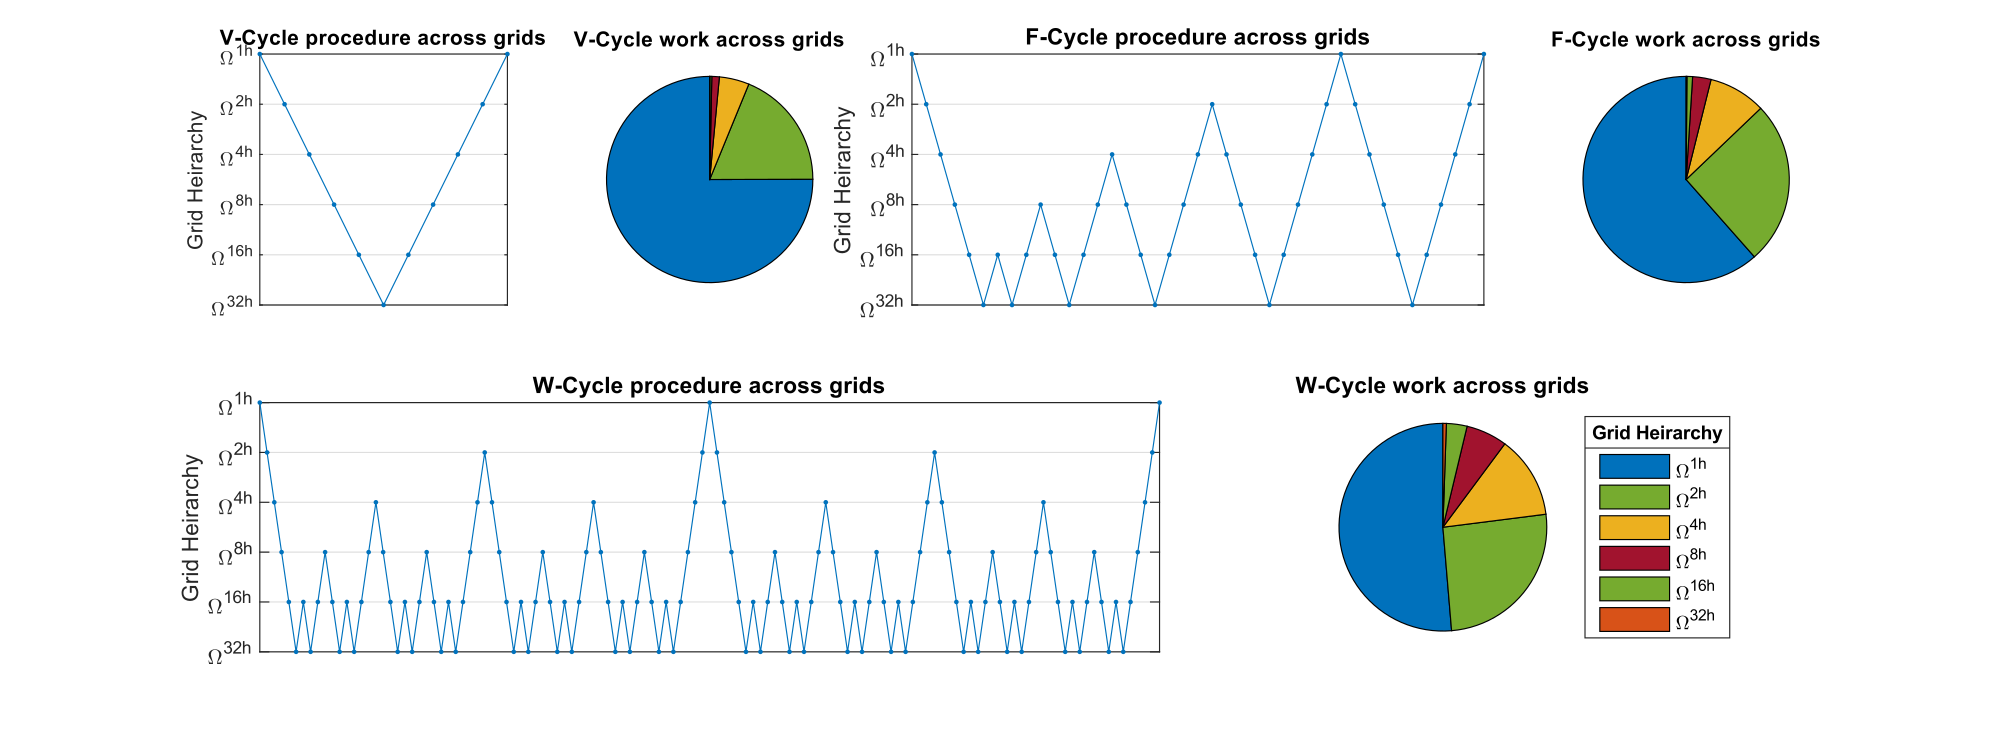
\includegraphics[width=\textwidth]{common_images/MultigridWork.png}
\caption{Различные циклы Многосеточного метода. \begin{small}(Источник: \url{https://commons.wikimedia.org/wiki/File:MultigridWork.svg})\end{small}}
\label{fig:multigrid}
\end{figure}

\subsubsection{Метод сопряженных градиентов \label{methods:conjugate_gradients}}
\paragraph{Прямой подход}
Данный метод относится к методам подпространства Крылова.
Пусть $\mathbf{A}$ - симметричная, положительно-определенная матрица, а $\mathbf{x_*}$ - решение исходной системы. Будем приближаться к решению \textit{сопряженными} шагами. \textit{Сопряженными} относительно матрицы $\mathbf{A}$ называются такие векторы $\mathbf{u}$ и $\mathbf{v}$, что  $\mathbf{u^T A v} = 0$. Решение можно представить через набор сопряженных векторов $P = \{ \mathbf{p_1}, ..., \mathbf{p_n} \}$, они образуют базис подпространстве Крылова \eqref{eq:krylov_subspace}. Тогда искомое решение имеет вид:
\begin{equation}
\mathbf{x_*} = \sum^n_{i=1} \alpha_i \mathbf{p_i}
\end{equation}
Домножим его на $\mathbf{A}$:
\begin{equation}
\mathbf{A x_*} = \sum^n_{i=1} \alpha_i \mathbf{A p_i}
\end{equation}
Домножим на $\mathbf{p_k^T}$, пользуясь сопряженностью $\mathbf{p}$:
\begin{equation}
\mathbf{p}^T_k \mathbf{A} \mathbf{x_*} = \alpha_k \mathbf{p_k}^T \mathbf{A} \mathbf{p_k}
\end{equation}
Воспользуемся \eqref{eq:linear_system}, выразим $\alpha_k$:
\begin{equation}
\alpha_k = \frac{\mathbf{p}^T_k \mathbf{b}}{\mathbf{p_k}^T \mathbf{A} \mathbf{p_k}}
\end{equation}
Для точного решения нужно найти $n$ базисных векторов $\mathbf{p}_k$ и коэффициентов $\alpha_k$.

\paragraph{Итерационный подход}
Если удачно выбрать несколько первых базисных векторов $\mathbf{p}_k$, можно не делать все $n$ шагов
для получения решения с нужной точностью. Итерационный подход рассматривает решение системы как задачу
минимизации функции
\begin{equation}
f(\mathbf{x}) = \frac{1}{2} \mathbf{x}^T \mathbf{A} \mathbf{x} - \mathbf{x}^T \mathbf{b}
\end{equation}
где минимум $\mathbf{x_*}$ cуществует, поскольку вторая производная $\nabla ^2 f(\mathbf{x}) = \mathbf{A}$ симметрична и положительно определена. Градиентом функции является невязка исходной задачи:
\begin{equation}
\nabla f(\mathbf{x}) = \mathbf{r} = \mathbf{Ax} - \mathbf{b}
\end{equation}
Возьмем начальное приближение решения $\mathbf{x_0}$. Так как мы ищем минимум функции, можно взять первым базисным вектором отрицательный градиент в точке $\mathbf{x_0}$:
\begin{equation}
\mathbf{p}_0 = \mathbf{b} - \mathbf{Ax}_0
\end{equation}
Cледующие шаги выбираются в направлении, сопряженном ко всем предыдущим базисным векторам:
\begin{equation}
\mathbf{p}_k = \mathbf{r}_k + \sum_{i < k} \frac {\mathbf{p}^T_i \mathbf{A r}_k}
{\mathbf{p}^T_i \mathbf{A p}_i} \mathbf{p}_i
\end{equation}
где $\mathbf{r}_k = \mathbf{b} - \mathbf{Ax}_k$ - текущая невязка. Так находится приближенное решение
$\mathbf{x}_{k+1} = \mathbf{x}_k + \alpha_k \mathbf{p}_k$.
\\ \\
Коэффициент $\alpha_k$ находится из минимизации $f(\mathbf{x}_{k+1})$ по параметру $\alpha_k$. Пользуемся $f(\mathbf{x}_{k+1}) = f(\mathbf{x}_k + \alpha_k \mathbf{p}_k) = g(\alpha_k)$, требуем $g'(\alpha) = 0$. Отсюда:
\begin{equation}
\alpha_k = \frac {\mathbf{p}^T_k (\mathbf{b} - \mathbf{A x}_k)} {\mathbf{p}^T_k \mathbf{A} \mathbf{p}_k}
\end{equation}
\par
Метод сопряженных градиентов может быть преобразован в форму, не требующую хранения в памяти всех базисных векторов $\mathbf{p}_k$. Сходимость метода оценивается в \cite{Golub}.
\par
Главный недостаток метода - матрица должна быть симметрична и положительно определена. В уравнении теплопроводности \eqref{eq:heat_equation_intro} эти требования выполняются. В системе \textit{функционала плотности} \eqref{eq:dhd_system_intro} они могут не выполняться. Поэтому необходимо рассмотреть другие методы, которые не накладывают такие ограничения.

\subsubsection{Метод обобщенных минимальных невязок (GMRES) \label{methods:gmres}}
Данный метод относится к методам подпространства Крылова.
Решение приближается через вектор в \textit{подпространстве Крылова} с минимальной невязкой. Подпространство строится по вектору невязки: $K_n = K_n(A, r_0)$, где $r_0 = b - Ax_0$, $x_0$ - начальное приближение. Точное решение приближается вектором $x_n \in K_n$, с которым невязка $r_n$ минимальна.
\par
Векторы $r_0, A r_0, \dots A^{n - 1} r_0 \in K_n$  могут быть практически линейно зависимыми. Удобнее построить ортонормированный базис $q_1,\dots q_n \in K_n$  с помощью \textit{итераций Арнольди} (процесс описан в \cite{saad2003iterative}). После этого решается задача минимизации нормы невязки и строится решение исходной системы. Базисные векторы $q_1, \dots q_n$  формируют матрицу $Q_n$, по которой раскладывается решение: $x_n = Q_n y_n$. В процессе \textit{итераций Арнольди} формируется верхняя матрица Хессенберга $\tilde H_n$ размерности $(n + 1) \times n$:

\begin{equation}
A Q_n = Q_{n+1} \tilde H_n
\end{equation}
Получим выражение нормы невязки для минимизации:
\begin{equation}
||r_n|| = ||A x_n - b|| = ||\tilde H_n y_n - Q^T_{n+1} b|| = ||\tilde H_n y_n - \beta e_1||
\end{equation}
Здесь мы воспользовались тем, что $Q_n$ образуется из ортонормированного базиса векторов. $e_1$ - первый базисный вектор в начальном базисе в $\mathbb{R}^{n+1}$. $\beta = ||b - A x_0||$. Таким образом, $x_n$ можно найти, минимизируя норму невязки:
\begin{equation}
r_n = \tilde H_n y_n - \beta e_1
\end{equation}
Данная задача сводится к задаче наименьших квадратов. Приведем алгоритм n-ой итерации метода GMRES:
\begin{enumerate}
\item Вычисление нового базисного вектора \textit{методом Арнольди}
\item Нахождение $y_n$, который минимизирует невязку $||r_n||$
\item Вычисление $x_n = Q_n y_n$
\item Повторение, если невязка недостаточно мала
\end{enumerate}

Метод GMRES может быть использован с произвольной обратимой матрицей. С увеличением размерности подпространства $K_n$ увеличивается объем используемой памяти. Поэтому раз в определенное количество итераций необходимо делать рестарт с новым приближенным решением.
\par
Подробное описание метода GMRES приводится в \cite{saad2003iterative}.

\subsubsection{Метод бисопряженных градиентов}
Метод сопряженных градиентов решает только системы с симметричной матрицей. Можно модифицировать его, чтобы снять это ограничение.
Данный метод ищет невязку в подпространстве Крылова \eqref{eq:krylov_subspace} $K(v, A)$, где вектор $v$ обычно берется нормированной невязкой начального приближения. Отличие от метода сопряженных градиентов заключается в том, что вектора проекций решения строятся ортогонально подпространству Крылова $K(w, A^T)$, где $w = b^* - A^T x_0^*$. Вектор $v$ должен быть ортогонален вектору $w$. Алгоритм метода приводится в \cite{saad2003iterative}.  

\subsubsection{Стабилизированный метод бисопряженных градиентов (BiCGStab) \label{methods:bicgstab}}
Данный метод разработан на основе \textit{метода бисопряженных градиентов} и \textit{метода GMRES}, чтобы улучшить стабильность сходимости. На каждом шагу бисопряженных градиентов решается система методом GMRES с рестартом на каждой итерации.
Подробнее данный метод описывается в \cite{saad2003iterative}.

\subsubsection{Предобуславливатели \label{methods:preconditioning}}
Оценки сходимости итерационных методов проведены в \cite{briggs2000multigrid}. Они показывают, что итерационные методы работают эффективно с хорошо обусловленной матрицей. Перед решением системы можно совершить линейное преобразование и решать \textit{предобусловленную} систему. 
\paragraph{Предобуславливателем} матрицы $\mathbf{A}$ называется такая матрица $\mathbf{M}$, что $\mathbf{M} \cdot \mathbf{A} \approx \mathbf{I}$, где $\mathbf{I}$ - единичная матрица. У $\mathbf{I}$ наилучшее число обусловленности: $\mu(\mathbf{I}) = 1$. Иначе говоря, $\mathbf{M} \approx \mathbf{A^{-1}}$. \textit{Алгоритмы подпространства Крылова} не используют саму матрицу, однако каждый из них можно модифицировать, чтобы решалась предобусловленная система $\mathbf{M} \cdot \mathbf{A} \cdot x = \mathbf{M} \cdot \mathbf{b}$ или $\mathbf{A} \cdot \mathbf{M} \cdot x = \mathbf{b} \cdot \mathbf{M} $.
\par
Для произвольного численного метода в качестве предобуславливателя можно эффективно использовать полную или неполную факторизацию Холецкого или LU (раздел \ref{methods:ilu}), поскольку они позволяют получить приближение обратной матрицы в явном виде.
В качестве предобуславливателя \textit{метода подпространства Крылова} можно использовать любой численный метод решения линейной системы. Достаточно сделать несколько итераций такого метода, чтобы примерное решение системы: $\mathbf{x} \approx \mathbf{A}^{-1} \mathbf{b}$. Подробнее использование предобуславливателей описано в \cite{Golub} и \cite{saad2003iterative}.

\section{Подходы к эффективной реализации алгоритмов \label{implementation}}
Для реализации численных методов решения уравнения теплопроводности \eqref{eq:heat_equation_intro} и системы функционала плотности \eqref{eq:dhd_system_intro} был выбран язык программирования Python 3 \cite{Python3}. Выбор этого языка связан с простотой написания и внесения изменений в код, а так же богатая экосистема вокруг него. При использовании возможностей библиотек трехмерный расчет становится достаточно быстрым для проведения исследований. Перечислим, какими библиотеками мы воспользовались:
\begin{itemize}
\item Арифметические операции для массивов, заранее скомпилированные в машинный код, из библиотеки Numpy \cite{Numpy}
\item Компиляция во время исполнения отдельных участков кода с помощью библиотеки Numba \cite{Numba}
\item Некоторые алгоритмы линейной алгебры из библиотеки Scipy \cite{Scipy}
\end{itemize}

С помощью данных подходов мы избавляемся от большого количества циклов и оперируем векторами и матрицами более абстрактно.

\subsection{Символьная математика \label{implementation:symbolic}}
В исследуемых задачах теплопроводности \eqref{eq:heat_equation_intro} и функционала плотности \eqref{eq:dhd_system_intro} все функции, заданные аналитически, считаются гладкими. В данной работе мы много раз сталкивались и еще столкнемся с необходимостью посчитать аналитический вид частных производных:
\begin{enumerate}
    \item для функций, используемых в системе функционала плотности из обобщенной свободной энергии
    \item для вычисления матрицы Якоби или ее действия в безматричном подходе (раздел \ref{methods:computing_jacobi})
    \item для тестирования при восстановлении задачи из известного решения (раздел \ref{implementation:convergence})
\end{enumerate}

Формулы, которые мы дифференцируем, могут быть очень сложными, и их реализация в коде приводила бы к ошибкам. Процесс аналитического дифференцирования можно автоматизировать. В данной работе используется библиотека Sympy \cite{Sympy}. Создаются объекты, представляющие математические переменные. Исходные формулы выражаются через них аналитически в коде. После этого библиотека может найти определенные частные производные. Затем эти производные арифметически упрощаются. Из них может быть сгенерирован код на Python 3 с использованием библиотеки Numpy. Кроме того, можно получить код формул на языке C для дальнейшей компиляции. Этот подход используется в разделе \ref{implementation:cuda}.
\subsection{Использование CUDA \label{implementation:cuda}}
В дальнейшем планируется реализовать численный метод для неявного моделирования системы функционала плотности в декартовых координатах в 3D. Такой расчет должен быть высокопроизводительным, так как размеры решаемой линейной системы увеличатся кубически по сравнению с одномерной задачей. Оптимизации такого расчета на Python будет недостаточно. 
\par
Для многократного ускорения расчета можно перенести вычисления на GPU с помощью технологии CUDA \cite{Cuda}. Этот подход требует написания низкоуровневого кода на языке C\texttt{++}. Так, нам приходится выбирать между удобством реализации и производительностью. 
\par
Среди преимуществ высокоуровневой реализации отдельно выделим использование символьной математики. В системе функционала плотности физическая модель конкретных жидкостей задается с помощью свободной энергии $f(n_i)$ из формулы \eqref{eq:chemical_potential_intro}. Для моделей, применяемых на практике, это обычно сложная формула. Для расчета такой модели по методу функционала плотности понадобится найти аналитически производные этой функции по $n_i$. Для неявного метода в матрице Якоби понадобятся еще и вторые производные. Поэтому внедрение новых физических моделей в программу может быть очень трудозатратным. С помощью символьной математики этот процесс можно автоматизировать. При этом нельзя жертвовать скоростью расчета.
\par
Рассмотрим, как можно совместить преимущества символьной математики с разработкой эффективного кода с помощью библиотеки PyCuda \cite{Pycuda}. Алгоритм схематично изображен на рис. \ref{fig:cuda_architecture}.
Процесс, запускаемый с CPU на GPU, в рамках терминов CUDA принято называть \textit{ядром}. PyCuda позволяет запускать ядра CUDA из Python. Воспользуемся Sympy для генерации кода на С и добавим нужные атрибуты для компилятора CUDA. Так можно автоматически генерировать код, зависящий от физической модели, и связывать его с общим кодом для всей численной схемы.
Другим преимуществом PyCuda является автоматизированное управление указателями на массивы, находящиеся на GPU. Это избавляет от необходимости управлять памятью вручную. 
\par
Вызовы ядра CUDA происходят из Python с помощью PyCuda. Этот подход позволяет разделить низкоуровневый код численной схемы и вспомогательные задачи, от которых не требуется высокой производительности. Код для CUDA генерируется и компилируется из Python один раз, поэтому не замедляет расчет. 
При этом значительно упрощается разработка вспомогательных задач, таких как тестирование.
\par
Данный подход позволяет разрабатывать и внедрять модели новых жидкостей исследователям без изменения кода программы. Со стороны пользователя достаточно просто задать уравнения, описывающие физическую модель, и запустить высокоэффективный расчет.
\par
В рамках данной работы реализована описываемая архитектура для неявной численной схемы уравнения теплопроводности в 3D. Реализация его для системы функционала плотности - тема планируемых исследований.
\begin{figure}[H]
\centering
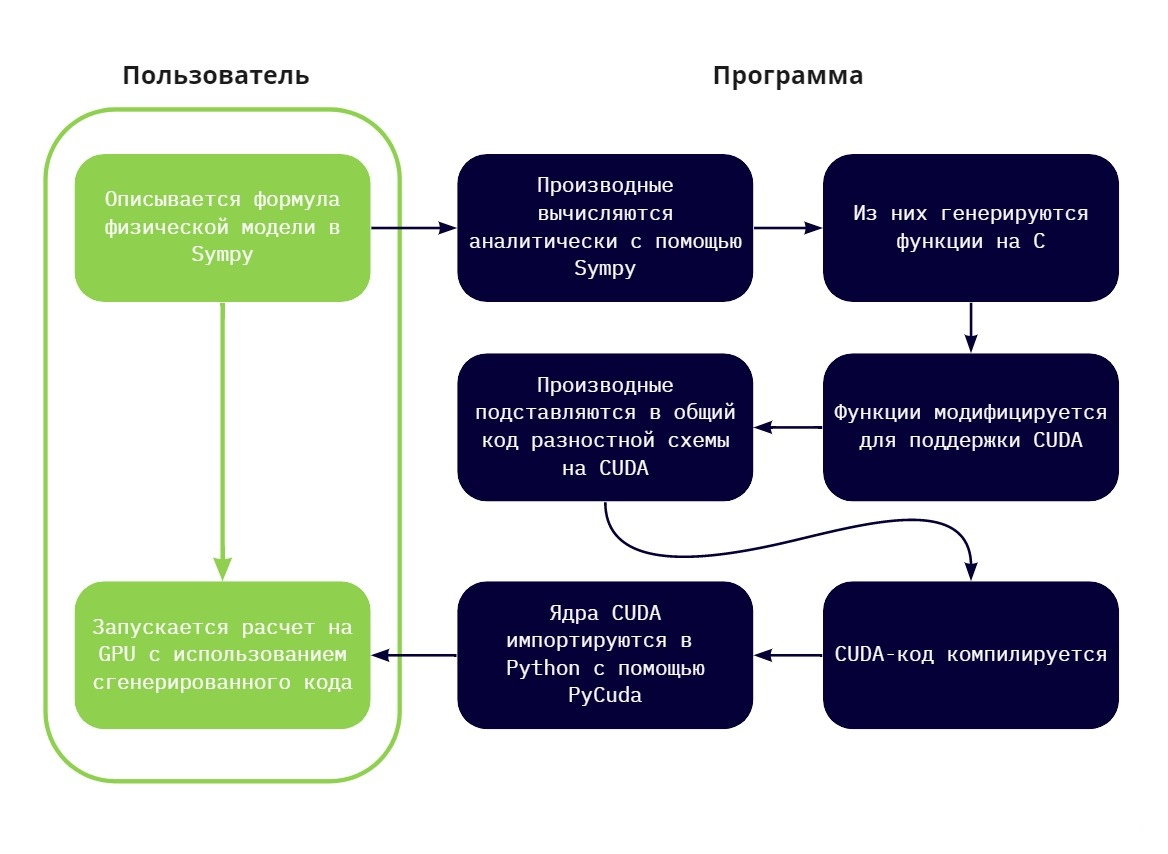
\includegraphics[width=\textwidth]{common_images/CUDA_architecture.jpg}
\caption{Архитектура программы с использованием PyCuda и Sympy}
\label{fig:cuda_architecture}
\end{figure}


\subsection{Вычисление матрицы Якоби \label{methods:computing_jacobi}}
Линейная система, которая решается в методе Ньютона, включает в себя матрицу Якоби. Рассмотрим разные подходы ее вычисления.

\subsubsection*{Прямой метод}
Можно получить явный вид матрицы Якоби: 
\begin{equation}
    J_{ij} = \frac{\partial F_i}{\partial u^n_j}
\end{equation}
Для этого нужно посчитать все частные производные аналитически. Можно делать это вручную или воспользоваться программами символьной математики, описанными в разделе \ref{implementation:symbolic}. Можно воспользоваться разреженной структурой матрицы, значительно уменьшая объем вычислений. Главный недостаток этого метода - формулы получаются очень большими.

\subsubsection*{}
Для \textit{методов подпространства Крылова} (раздел \ref{methods:linear_solvers}) достаточно знать только, как матрица действует на произвольный вектор. Сама матрица в явном виде при этом не нужна. Вместо нее мы можем создать оператор, действие которого на произвольный вектор будет давать такой же результат, как при умножении матрицы на этот вектор. Получим такой оператор:
\begin{equation}
J(x) = \frac {\partial F(x)} {\partial x}
\end{equation}
Умножение матрицы Якоби на вектор с линейной точностью равно нахождению изменению вектора $F(X)$ в направлении этого вектора:
\begin{equation}
dF(x) = J \cdot dx
\end{equation}
\begin{equation}
J \cdot a \approx dF(x) \vert_{dx = a}
\end{equation}

\subsubsection*{Разностный метод}
Вычислим $dF$ численно как производную по направлению:
\begin{equation}
dF = \frac{F(x + \varepsilon a) - F(x)}{\varepsilon}
\end{equation}
Точность такого метода настраивается выбором малого параметра $\varepsilon$. С разностным методом вычисления матрицы Якоби мы получаем метод, позволяющий решить нелинейную систему уравнений, указав только вид функции $F(x)$ для метода Ньютона. Такой метод называется \textit{JFNK-метод} (Jacobi-Free Newton-Krylov). Его свойства сходимости исследуются в \cite{JFNK}.

\subsubsection*{Аналитический метод}
Можно вычислить действие оператора Якоби, используя правило дифференцирования сложной функции. Исследуемую функцию $F$ запишем в общем виде: 
\begin{equation}
F :=L(u^n) -\varphi(u^{n-1}, x_i, t) = 0
\end{equation}
где $u^n$ - искомый вектор переменных в момент времени $t_n$, $L$ - гладкая функция, зависящая от них. В функции $\varphi$ собраны все члены, которые на зависят от неизвестного вектора $u^n$.
Дифференцируем:
\begin{equation}
dF = \frac{\partial L(u^n)} {\partial u^n} du^n
\end{equation}
Частные производные функции $L$ для конкретной задачи могут быть тоже упрощены с помощью правила дифференцирования сложных функций и вычислены с помощью символьной математики. Пример применения данного метода есть в разделе \ref{dhd:features}. Данный способ сложнее разностного метода в реализации, однако он точнее. Поэтому разностный метод можно использовать для тестирования реализации данного способа.

\subsection{Предобуславливание безматричного метода \label{implementation:operator_preconditioning}}
Численные методы решения СЛАУ используют предобуславливатели (раздел \ref{methods:preconditioning}). Для вычисления предобуславливателя нужна матрица Якоби. Но мы используем методы \textit{подпространства Крылова}, где мы не храним явный вид этой матрицы. Поэтому нужен алгоритм ее получения из безматричного представления. 
\par
Получить явный вид можно, используя результат умножения оператора Якоби на вектор $\delta^i$, у которого равны нулю все элементы, кроме $i$:
\begin{equation}
\begin{cases}
\delta^i_i = 1
\\
\delta^i_{j \neq i} = 0
\end{cases}
\end{equation}
Действие оператора Якоби на $\delta^i$ дает $i$-й столбец матрицы $J$. Для получения явного вида $J$ размерности $N \times N$ нужно сделать $N$ перемножений. 

\subsubsection*{Оптимизация вычисления}
Существует подход, позволяющий вычислить вид матрицы Якоби, подействовав оператором на вектор конечное количество раз независимо от размерности матрицы. Для этого матрица должна быть разреженной, и мы должны знать ее структуру. Рассмотрим простейший случай: пусть матрица тридиагональна \eqref{mat:tridiagonal}. Тогда $i$ строка матрицы будет влиять только на $i$, $i + 1$ и $i - 1$ элементы вектора $c$ в уравнении $A \cdot b = c$. Пусть вектор $b$ будет иметь вид:
\begin{equation}
\begin{cases}
b_i = 1, \quad i \bmod  3 = 0 \\
b_i = 0, \quad i \bmod  3 \neq 0
\end{cases}
\end{equation}
где $\bmod$ означает остаток от деления. Тогда результат умножения $c$ будет содержать в себе всю информацию о каждом третьем столбце матрицы Якоби. После этого нужно два раза повторить циклический сдвиг значений вектора $b_i$ и получить информацию о недостающих $2/3$ столбцах матрицы Якоби.

\subsubsection*{Оптимизация применения}
Пусть нам необходимо вычислить предобуславливатель на каждом шагу по времени. Тогда сводится на нет преимущество в производительности от операторного подхода, поскольку на каждом шагу мы вычисляем матрицу в явном виде.

Чтобы сохранить сильные стороны безматричного подхода, рассмотрим такую оптимизацию. Предположим, что матрица Якоби не сильно меняется от шага к шагу по времени. Тогда мы можем переиспользовать один предобуславливатель в течение нескольких следующих итераций. Поскольку это предположение никак не подкреплено теоретически, необходимо ввести параметр $P$, отвечающий за пересчет предобуславливателя. Будем пересчитывать предобуславливатель, если метод решения СЛАУ сделал больше $P$ итераций. Подбирается оптимальное значение параметра $P$, соблюдающее баланс между частым пересчетом предобуславливателя и долгой сходимостью итерационного метода. Начать расчет можно вообще без предобуславливателя. Посчитать его нужно будет, только если итерационный метод будет сходиться дольше, чем за $P$ итераций.
\par
В медленных процессах матрица Якоби действительно меняется слабо, и предобуславливатель можно переиспользовать довольно долго. Такой подход позволяет существенно сократить вычислительные затраты.

\subsection{Стратегии тестирования \label{implementation:testing}}
Реализация любого численного алгоритма - это в том числе написание программы. В ней можно допустить множество ошибок – от неправильно поставленного знака до опечатки. Поэтому важно с самого начала правильно заложить в программу стратегии тестирования. Тесты позволяют быть уверенным, что изменения внесены в алгоритм корректно и ничего не сломалось.
\par
В этой главе мы рассмотрим подходы, используемые для тестирования реализованных программ в данной работе. Некоторые из подходов реализованы в виде автоматических тестов, другие предоставляют отчет для оценки.

\paragraph{Сравнение с задачей с постоянными коэффициентами}
Если реализованы алгоритмы решения линейной и нелинейной задачи, можно сравнить их результаты, взяв нелинейный коэффициент постоянным. Рассмотрим этот тест на примере уравнения теплопроводности\eqref{eq:heat_equation_intro}. Возьмем $\alpha = const$, задача станет линейной. В случае явного метода ход решения останется таким же. Изменения в ходе решения неявного метода станут значительными. Больше не нужно решать нелинейную систему методом Ньютона (раздел \ref{methods:newton}). Остается решить систему $\mathbf{F} \cdot \mathbf{u}^{n+1} = \mathbf{b}$, где $\mathbf{F} = const$. На каждом шагу по времени нужно решить одну систему линейных уравнений. Результаты данного метода должны совпадать с результатами нелинейного алгоритма с $\alpha(u) = const$ с точностью порядка аппроксимации.

\paragraph{Тестирование операторов производной}
Оператор второй производной по пространству в коде можно выразить отдельной функцией. Тогда его будет удобно тестировать отдельно от всей задачи.
Тестирование линейной задачи проводится на полиномах и собственных функциях. 
\begin{enumerate}
\item Полиномы 1 и 2 степени должны дифференцироваться точно, так как производная по пространству аппроксимируется со 2-м порядком. Ошибка вносится только конечной машинной точностью, поэтому она увеличивается при уменьшении шага сетки. Полиномы степени $n > 2$ дифференцируются с точностью порядка аппроксимации.
\item Собственные функции под действием оператора умножаются на известное собственное значение: $D^2_x \cdot u_{eig} = \lambda \cdot u_{eig} + O(h^p)$. Собственными функциями оператора второй производной являются $sin (x)$ и $cos(x)$. 
Разность должна сходиться к нулю с порядком аппроксимации $p$: $D^2_x \cdot u_{eig} - \lambda \cdot u_{eig} = O(h^p)$
\end{enumerate}

\paragraph{Сравнение с явным методом}
Явный и неявный методы должны сходиться к одному и тому же решению с ошибкой порядка аппроксимации. Можно сравнивать решения, полученные этими методами на одной и той же сетке в одинаковый момент времени.

\paragraph{Задачи меньшей размерности}
Ход решения трехмерной задачи качественно не отличается от двумерной. Можно поставить задачу большей размерности так, что начальные, граничные условия и источник не будут зависеть от одной из координат. Тогда решаемая задача на трехмерной сетке сведется к двумерной. Мы сможем сравнить их решения. Ошибка может появиться из-за конечной машинной точности или граничных условий, однако они будут порядка аппроксимации.
\par
Данный тест позволяет сначала безошибочно реализовать одномерную задачу, потому двумерную, а затем трехмерную.

\paragraph{Кросс-валидация}
Можно сравнить результаты с другой программой, реализующей ту же самую физическую модель.

\paragraph{Проверка законов сохранения}
Если численный метод консервативный, то в нем должны выполняться законы сохранения на дискретном уровне. Например, интегральная масса в системе функционала плотности \eqref{eq:dhd_system_intro} сохраняется, если нет источников и потока через границы. На каждом шагу можно проверять закон сохранения массы: 
\begin{equation}
m = \int_{D} \rho(\mathbf{x}) d\mathbf{x}
\end{equation}

\subsubsection*{Оценка сходимости \label{implementation:convergence} }
В главе \ref{methods} были рассмотрены численные методы с порядком сходимости $O(\tau, h^2)$ или $O(\tau^2, h^2)$. Исследование сеточной сходимости позволяет оценить, насколько близок реальный порядок сходимости к теоретическому. Для этого одинаковая задача решается на разных сетках с последовательно уменьшающимся шагом. 
\par
Шаг по времени $\tau$ в исследовании сеточной сходимости нужно брать постоянным. Он делится пропорционально $h^2$, если аналитический порядок $O(\tau, h^2)$. Таким образом можно погасить вклад ошибки первого порядка по $\tau$. Если исследуется схема с порядком $O(\tau^2, h^2)$, $\tau$ делится пропорционально $h$.
\par
Рассмотрим 3 метода вычисления порядка сходимости. В случае правильной реализации задачи, все 3 покажут одинаковый порядок. Отличие в результатах может указывать на типичные ошибки в реализации.
\paragraph{Сравнение с аналитическим решением}
Численную задачу можно получить из заранее выбранной формулы - решения. Из нее вычисляются начальные и граничные условия, а также источник. После этого аналитическое решение сравнивается с численным. Это прямой метод нахождения ошибки. Его недостаток в том, что нужно вручную вычислить аналитические производные. Этот процесс можно автоматизировать с помощью символьной математики, раздел \ref{implementation:symbolic}. В результате работы данного теста формируется график зависимости нормы ошибки от шага сетки. Используется норма $L_2$ в конкретный момент времени по всему пространству. Поскольку ожидается ошибка $\varepsilon = C \cdot h^2$, график строится в логарифмическом масштабе: $\log_{10} \varepsilon = 2 \log_{10} h + \log_{10} C$. В тех же осях откладывается прямая линия $y = 2x$ для сравнения угла наклона. 
\par
Данный метод - самый точный из трех рассматриваемых, однако для его применения нужно знать аналитическое решение.

\paragraph{Порядок по мелкой сетке}
Решение на самой мелкой сетке принимается за точное решение. Другие решения сравниваются с ним. График ошибки относительно самой мелкой сетки строится на одних осях с графиком ошибки по предыдущему методу. Возможна ситуация, когда этот признак дает хороший порядок сходимости, а признак сравнения с аналитическим решением - нет. Это значит, что решения сходятся, но не к аналитическому решению. Скорее всего, допущена одна из ошибок:
\begin{itemize}
\item задача получена из аналитического решения неправильно
\item численный метод аппроксимирует другую задачу
\item решение берется не в нужных точках
\end{itemize}

\paragraph{Порядок по 3 сеткам}
Пусть $\tilde u$ - точное решение, а $u_h$ - численное решение на сетке с шагом $h$. Ищем порядок сходимости $p$, на сетках с шагом $h, \alpha h, \alpha^2 h$.
\begin{equation}
u_h = \tilde u + O(h^p) \approx \tilde u + C \cdot h^p
\end{equation}
Поэтому $|| u_h - u_{\alpha h} || \approx (1 - \alpha^p) \cdot ||C \cdot h^p||$.
\begin{equation}
\frac {||u_h - u_{\alpha h}||} {||u_{\alpha h} - u_{\alpha^p h}||} \approx \frac {1 - \alpha^p} {\alpha^p \cdot (1 - \alpha^p)} = \frac{1}{\alpha^p}
\end{equation}
Можно выразить порядок сходимости: 
\begin{equation}
p = log_\alpha \frac {||u_{\alpha h} - u_{\alpha^p h}||} {||u_h - u_{\alpha h}||}
\end{equation}
\subsection*{}
Описанные методы проверки сеточной сходимости собраны в одной программе. Она была использована для всех численных методов, реализованных в рамках данной работы. Примеры ее использования приведены в главах, посвященных конкретным задачам: \ref{heat:convergence} для уравнения теплопроводности и \ref{dhd:convergence} для системы функционала плотности.

\section{Исследование уравнения теплопроводности \label{heat}}
Целью данной главы является широкое рассмотрение подходов для решения нелинейных систем в одномерной, двумерной и трехмерной постановке.
Методы из главы \ref{methods} сравниваются, чтобы выбрать самые подходящие для решения системы функционала плотности. Сравнение проводится на упрощенной задаче \textemdash скалярном нелинейном уравнении теплопроводности. По аналогии с системой функционала плотности она включает в себя первую производную по времени и старшие производные по пространству с нелинейным коэффициентом.
\subsection{Постановка задачи}
Решается скалярное уравнение теплопроводности с нелинейным коэффициентом в кубической области $D \subset \mathbb{R^d}$, $t \in (0, T)$. Размерность пространства $d = \overline{1 \dots 3} $.
\begin{equation} \label{eq:heat_equation}
\frac{\partial u}{\partial t}+ \frac{\partial }{\partial x_i} \left( \alpha (u) \frac{\partial u}{\partial x_i} \right) = \nu(x_i, t)
\end{equation}
где $\nu(x_i, t)$ и $\alpha(u)$ - гладкие аналитические функции. Неизвестная функция $u(x_i, t)$ - гладкая.
\par
Задаются начальные условия:
\begin{equation} \label{eq:initial_condition_scalar}
u(x_i, t) \vert _{t = 0} = u_0(x_i)
\end{equation}
В качестве граничных условий рассматриваются \textit{условия Дирихле} или \textit{условия Неймана}:
\paragraph{условия Дирихле}
\begin{equation} \label{eq:dirichlet_heat}
u \vert_{\partial D} = \varphi(x_i, t)
\end{equation}
\paragraph{условия Неймана}
\begin{equation} \label{eq:neumann}
    \left. \frac{\partial u}{\partial n} \right \vert_{\partial D} = \varphi(x_i, t)
\end{equation}
где $n$ - вектор нормали к границе $\partial D$.
\subsection{Дискретизация}
Для аппроксимации производных по пространству пользуемся методом центральных разностей из раздела \ref{methods:space_derivative}. Таким образом, мы получаем 2-ой порядок аппроксимации по пространству. Рассмотрим, как этот порядок сохраняется в граничных точках.
\par
Границу области $D$ можно расположить по-разному относительно сетки в зависимости от граничных условий. Это позволяет избежать интерполяцию граничных условий и потерю точности. Разные варианты расположения границы показаны на рис. \ref{fig:heat_bound}. В случае \textit{граничных условий Дирихле} известно значение на границе. Поэтому удобно взять точку сетки на границе. В случае \textit{граничных условий Неймана} известна производная на границе. Можно аппроксимировать ее со вторым порядком. Для этого нужно взять две соседние точки сетки, равноудаленные от границы. 
\begin{figure}[H]
\centering
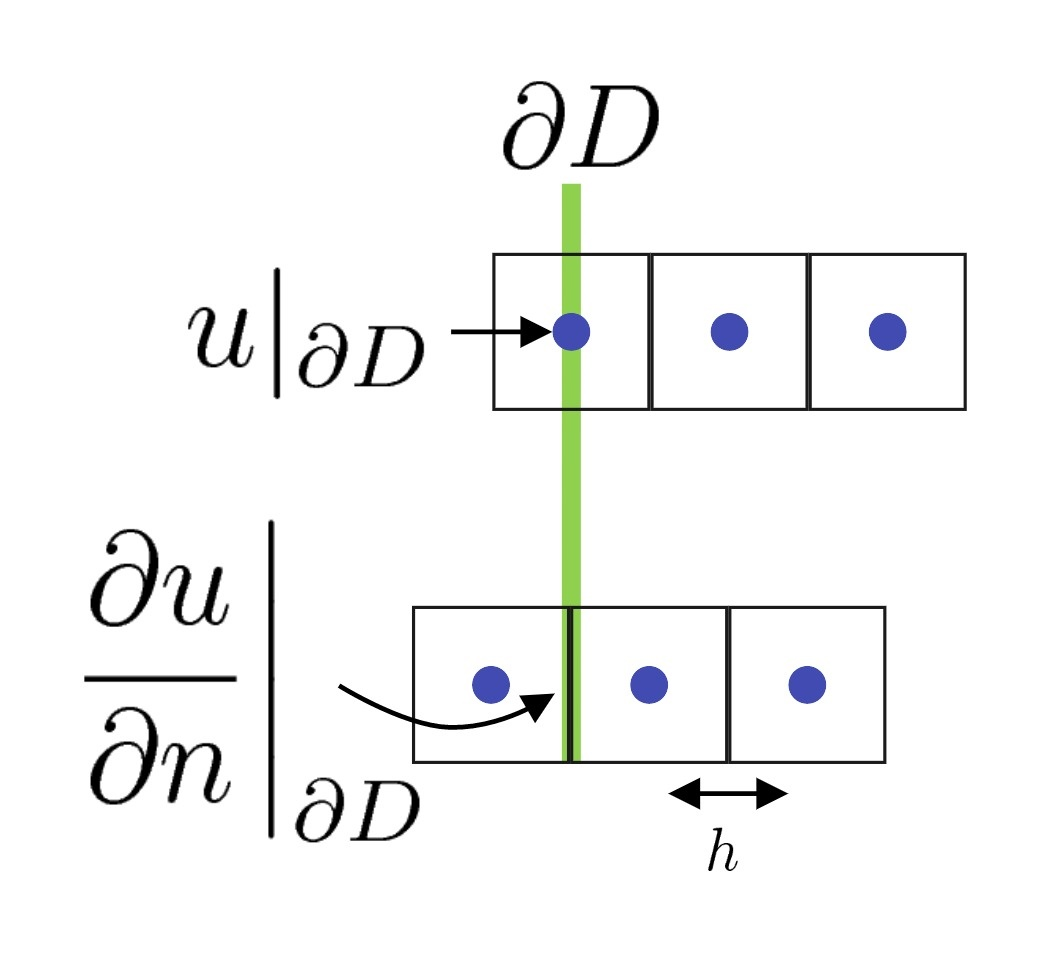
\includegraphics[width=.4\textwidth]{common_images/dirichlet_neumann.jpg}
\caption{Аппроксимация граничных условий. Синим цветом обозначены точки пространства, где ищется численное решение. Зеленым цветом обозначена граница.}
\label{fig:heat_bound}
\end{figure}
\subsection{Особенности реализации численных схем}
В рамках данной работы были реализованы программы, решающие уравнение теплопроводности \eqref{eq:heat_equation} в 1D, 2D и 3D. Поскольку реализовано большое количество похожих задач, отличающихся в деталях, сначала выпишем общие характеристики для всех решенных задач. Если не указано обратное, используется собственная реализация алгоритма.
Общие характеристики:
\begin{itemize}
\item Используем граничные условия Дирихле \eqref{eq:dirichlet_heat} и Неймана \eqref{eq:neumann}
\item Нелинейная система решается методом Ньютона (раздел \ref{methods:newton})
\item Отдельно реализованы линейная $\alpha(u) = const$ и нелинейная постановки задачи
\item Каждая задача решается явным и неявным по времени методом (раздел \ref{methods:time_integration})
\end{itemize}
Рассмотрим особенности реализации конкретных задач:
\paragraph{Одномерная задача}
\begin{itemize}
\item Неявное интегрирование по времени реализовано 3-мя способами: методом Эйлера, методом Кранка-Николсона и трехточечным методом второго порядка
\item Везде СЛАУ решается алгоритмом прогонки (раздел  \ref{methods:tridiagonal})
\item Система не предобуславливается
\end{itemize}

\paragraph{Двумерная задача}
\begin{itemize}
\item Кроме явной и неявной схемы, реализована схема переменных направлений (раздел \ref{methods:alternate_directions})
\item Предобуславливатель - метод ILU, реализация из Scipy (раздел \ref{methods:ilu})
\item Реализованы точный, численный и аналитический алгоритмы вычисления матрицы Якоби (раздел \ref{methods:computing_jacobi})
\end{itemize}

\paragraph{Трехмерная задача}
\begin{itemize}
\item Кроме явной и неявной схемы, реализована трехмерная схема переменных направлений, чтобы убедиться в ее неустойчивости
\item В неявном методе СЛАУ решается методом сопряженных градиентов
\item Предобуславливатель - разреженный метод LU (реализация из Scipy) и многосеточный метод (раздел \ref{methods:multigrid})
\item Расчет ведется на GPU с помощью PyCuda 
\end{itemize}
В двумерной и трехмерной постановках использовались не только указанные предобуславливатели, кроме них пробовались в качестве предобуславливателей все алгоритмы, описанные в главе \ref{methods}, однако вынесенные в список алгоритмы оказались наиболее производительными.

\subsubsection*{Особенность исследования сеточной сходимости}
Для правильной оценки нужно сравнивать значения в одни и те же моменты времени и в одних и тех же точках пространства. Поэтому более мелкие сетки должны точно проецироваться на самую крупную (рис. \ref{fig:convergence_bounds}). Для задачи с \textit{граничными условиями Дирихле} \eqref{eq:dirichlet_heat} шаг по пространству $h$ нужно делить в 2 раза, чтобы граничные точки попадали в себя. Для \textit{граничных условий Неймана} \eqref{eq:neumann} необходимо делить шаг по пространству в 3 раза. Первая точка находится на $\frac{h}{2}$ за границей, поэтому проецируется только внутренняя область.
\begin{figure}[H]
\centering
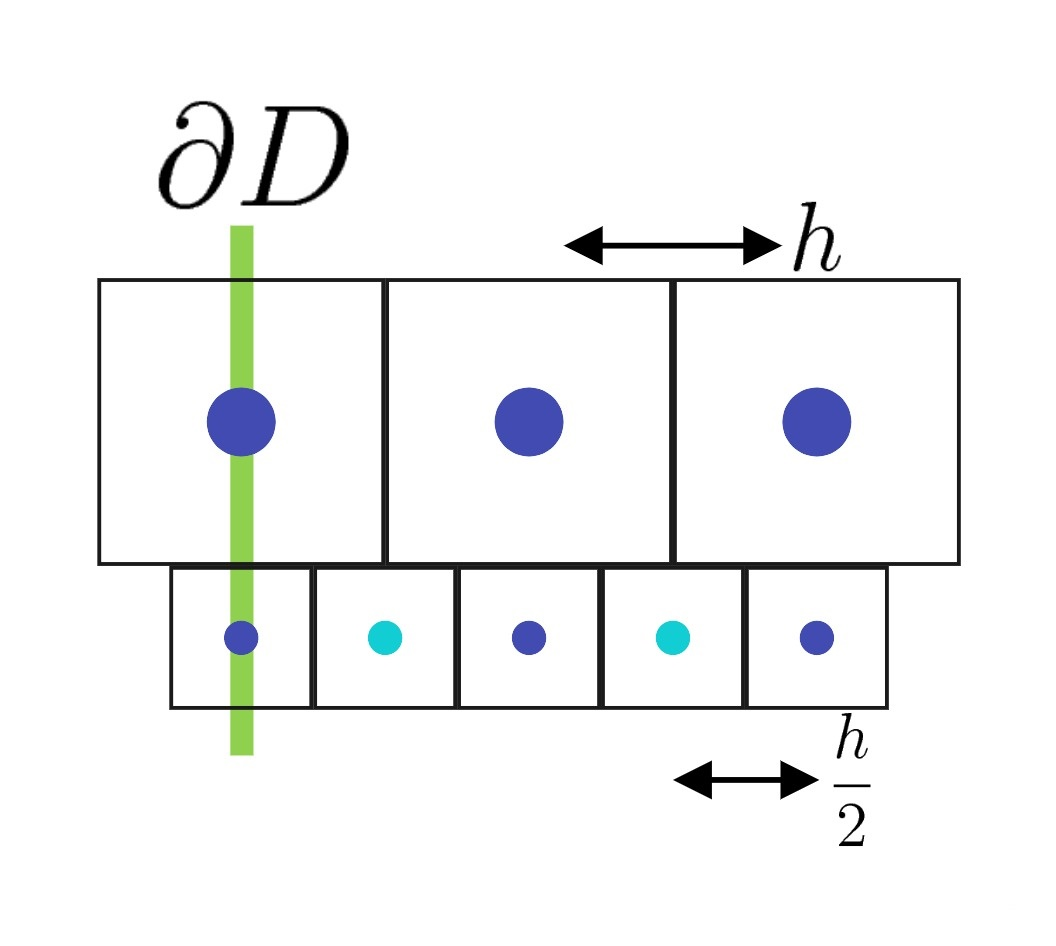
\includegraphics[width=.5\textwidth]{common_images/dividing_dirichlet.jpg}\hfill
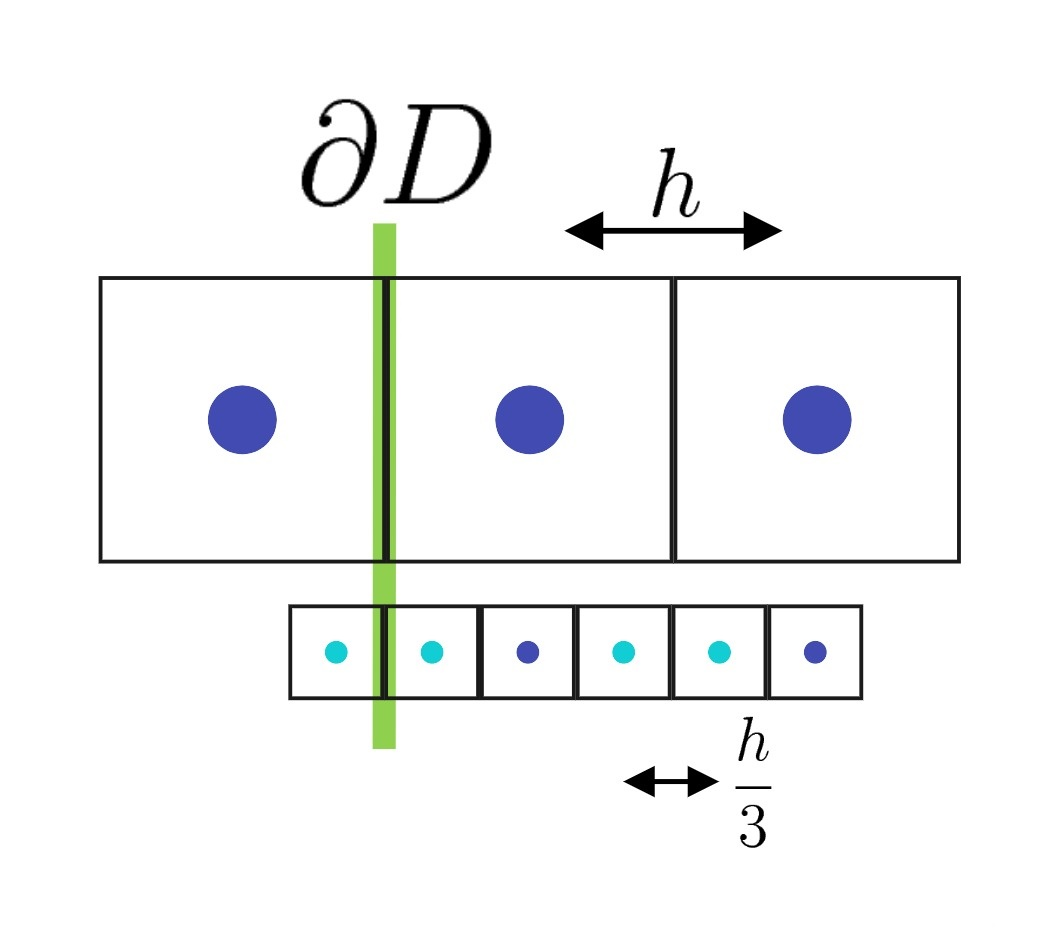
\includegraphics[width=.5\textwidth]{common_images/dividing_neumann.jpg}
\caption{Уменьшение сетки для граничных условий Дирихле (слева) и Неймана (справа). Темно-синим цветом выделены точки, проектирующиеся на более грубую сетку.}
\label{fig:convergence_bounds}
\end{figure}


\subsection{Численные эксперименты}
Исследование уравнения теплопроводности не является конечной целью данной работы. На его примере мы исследовали подходы, которые позже были использованы для более сложной системы функционала плотности. Поэтому все численные эксперименты с ним можно свести к исследованию корректности численных методов и их сходимости. Поскольку такие  эксперименты были проведены для каждой из описываемых задач, ограничимся приведением в данной работе только этих:
\begin{itemize}
\item Описание автоматического тестирования
\item Исследование сходимости метода переменных направлений в 2D
\item Сравнение результатов 2D и 3D расчетов
\item Исследование сходимости неявного метода в 3D
\end{itemize}
Для экспериментов, описанных ниже, используются граничные условия Дирихле. Задача решается в кубе $D = [0; 1]\times [0;1] \times [0;1]$, $t \in [0; 0.5]$. Мы формулируем постановку задачи на основе известной формулы, которая считается решением. Из нее вычисляются начальные и граничные условия, а также вычисляется вид источника. Во всех расчетах используется число Куранта:
\begin{equation}
\frac{\tau}{h^2} = 15
\end{equation}

\subsubsection{Автоматическое тестирование}
Для каждой задачи реализованы методы автоматического тестирования, описанные подробно в главе \ref{implementation:testing}:
\begin{itemize}
\item Сравнение линейной и нелинейной задачи
\item Тестирование операторов производной
\item Сравнение решения по разным методам для одной задачи
\end{itemize}

\subsubsection{Исследование сеточной сходимости 2D}
\paragraph{Постановка эксперимента}
В качестве решения используется формула:
\begin{equation}
u(x, y, t) = 2 + \sin \left(\pi \cdot \left( 0.5x + 0.25y - t\right) \right)
\end{equation}
В качестве нелинейного коэффициента используется:
\begin{equation}
\alpha(u) = \frac{u^{2} \left(\cos{\left(u \right)} + 2\right)}{9}
\end{equation}
Разобьем область по пространству и времени равномерными сетками. Минимальное количество точек в пространстве по каждому направлению - 21. Шаг по времени $\tau$ будем делить пропорционально $h^2$.

\paragraph{Применение символьной математики}
Если бы не действие нелинейного коэффициента $\alpha$, выбранное решение было бы собственной функцией для уравнения теплопроводности. Однако чтобы получить такое решение для нелинейного уравнения, источник должен постоянно действовать определенным образом. Чтобы найти вид источника, нужно подставить $\alpha$ и $u$ в уравнение теплопроводности. Выпишем вид источника, полученный с помощью символьной математики:
\begin{equation}
\begin{split}
\nu & (x, y, z, t) = 
\\ 
&- 0.0347222222222222 \pi^{2} \left(\sin{\left(\pi \left(- t + 0.5 x + 0.25 y\right) \right)} + 2\right)^{2}  \cdot 
\\ 
& \cdot \left(\cos{\left(\sin{\left(\pi \left(- t + 0.5 x + 0.25 y\right) \right)} + 2 \right)} + 2\right) \sin{\left(\pi \left(- t + 0.5 x + 0.25 y\right) \right)} -
\\
& -0.0347222222222222 \pi^{2} \left(\sin{\left(\pi \left(- t + 0.5 x + 0.25 y\right) \right)} + 2\right)^{2} \cdot 
\\
& \cdot  \sin{\left(\sin{\left(\pi \left(- t + 0.5 x + 0.25 y\right) \right)} + 2 \right)} \cos^{2}{\left(\pi \left(- t + 0.5 x + 0.25 y\right) \right)} +
\\
& + 0.0694444444444444 \pi^{2} \left(\sin{\left(\pi \left(- t + 0.5 x + 0.25 y\right) \right)} + 2\right)  \cdot
\\
& \cdot \left(\cos{\left(\sin{\left(\pi \left(- t + 0.5 x + 0.25 y\right) \right)} + 2 \right)} + 2\right) \cos^{2}{\left(\pi \left(- t + 0.5 x + 0.25 y\right) \right)} -
\\
& - \pi \cos{\left(\pi \left(- t + 0.5 x + 0.25 y\right) \right)}
\end{split}
\end{equation}

\paragraph{Результаты}
На рис. \ref{fig:heat2d_time_error} справа приведен график зависимости нормы ошибки от шага в последний момент времени задачи. Слева приведена зависимость нормы ошибки от времени. Везде используется норма $L_2$.
\begin{figure}[H]
\centering
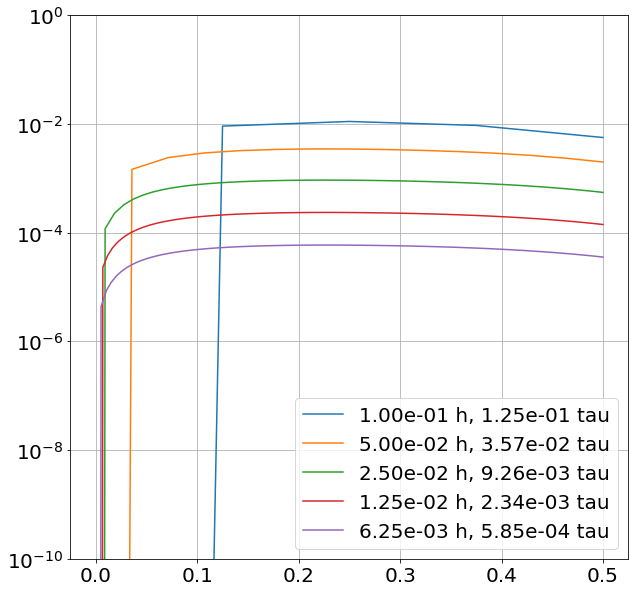
\includegraphics[width=.5\textwidth]{heat2d/time_error.png}\hfill
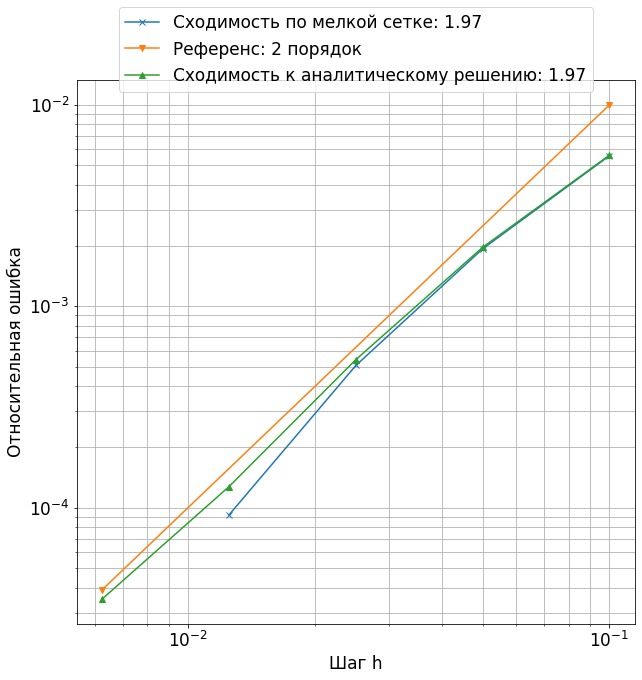
\includegraphics[width=.5\textwidth]{heat2d/convergence2d.png}
\caption{Зависимость нормы ошибки от времени (слева), зависимость нормы ошибки от шага сетки в последний момент расчета (справа)}
\label{fig:heat2d_time_error}
\end{figure}

Рассмотрим решения и ошибки в последний момент времени на рис. \ref{fig:heat2d_field}:

\begin{figure}[H]
\centering
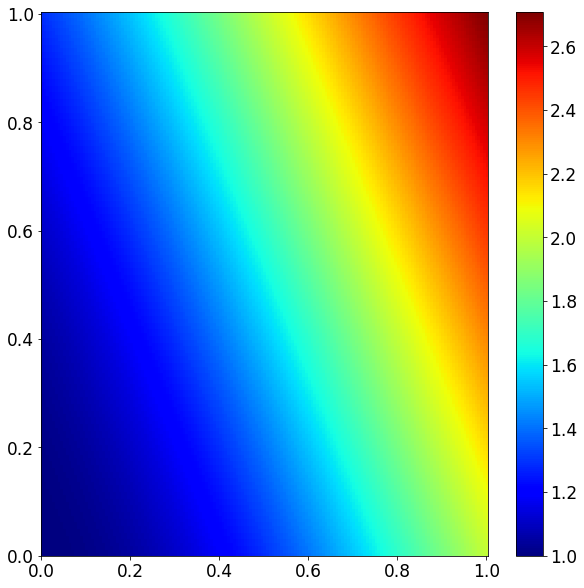
\includegraphics[height=.45\textwidth]{heat2d/solution.png}
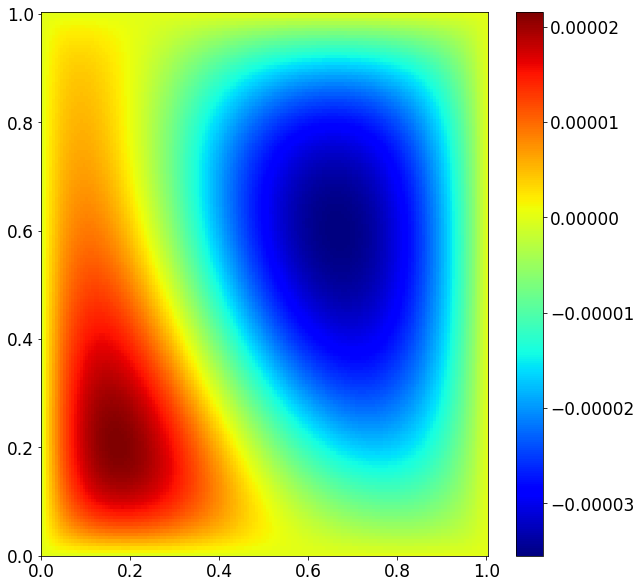
\includegraphics[height=.45\textwidth]{heat2d/error.png}
\caption{Решение (слева) и относительная ошибка (справа) на самой точной сетке из 161 точки по $x$ и $y$.}
\label{fig:heat2d_field}
\end{figure}



\subsubsection*{Сравнение результатов 2D и 3D расчетов}
Будем решать в трехмерной постановке двумерную задачу, как предложено в разделе \ref{implementation:testing}. Это позволит убедиться, что 2D и 3D расчеты согласованы и сходятся к одному и тому же решению.
\paragraph{Постановка численного эксперимента}
В качестве решения, из которого с помощью символьной математики ставится задача (раздел \ref{implementation:symbolic}), возьмем формулу:
\begin{equation}
u(x, y, t) = 2 + \sin \left(\pi \cdot \left( 0.5x + 0.25y - t\right) \right)
\end{equation}
В качестве нелинейного коэффициента возьмем:
\begin{equation}
\alpha(u) = \frac{u^2}{9}
\end{equation}
Двумерную задачу будем решать методом переменных направлений, а трехмерную - полностью неявным методом. Разобьем область равномерными сетками по пространству и времени. Для сеток по пространству используется 81 точка по каждому направлению. По времени пространство разбивается 215 точками.

\paragraph{Результаты} Проекцию по оси $z$ для сравнения берем посередине: $z = 0.5z_{max}$. 
Приведем графики решения 2D задачи и проекции решения 3D задачи на рис. \ref{fig:compare_2d_3d_fields}:
\begin{figure}[H]
\centering
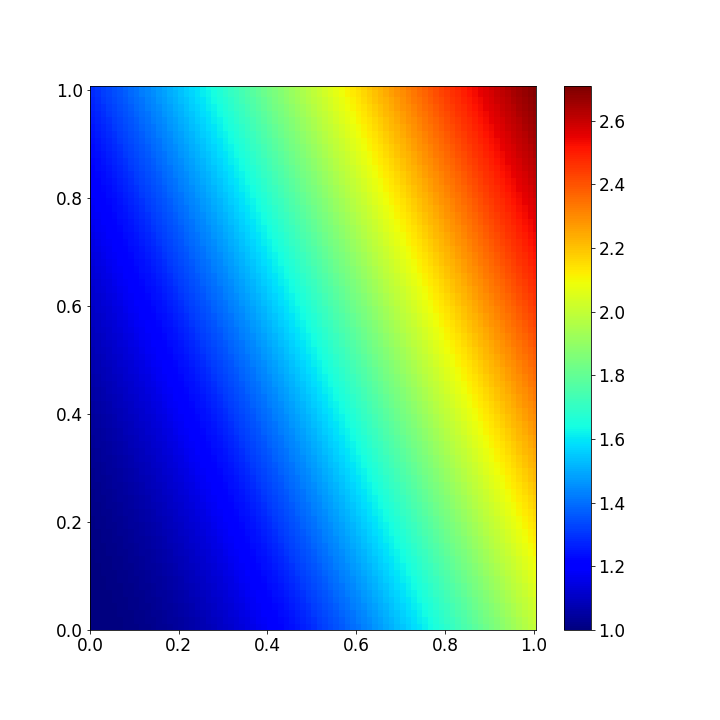
\includegraphics[width=.5\textwidth]{compare_2d_3d/field3d_80.png}\hfill
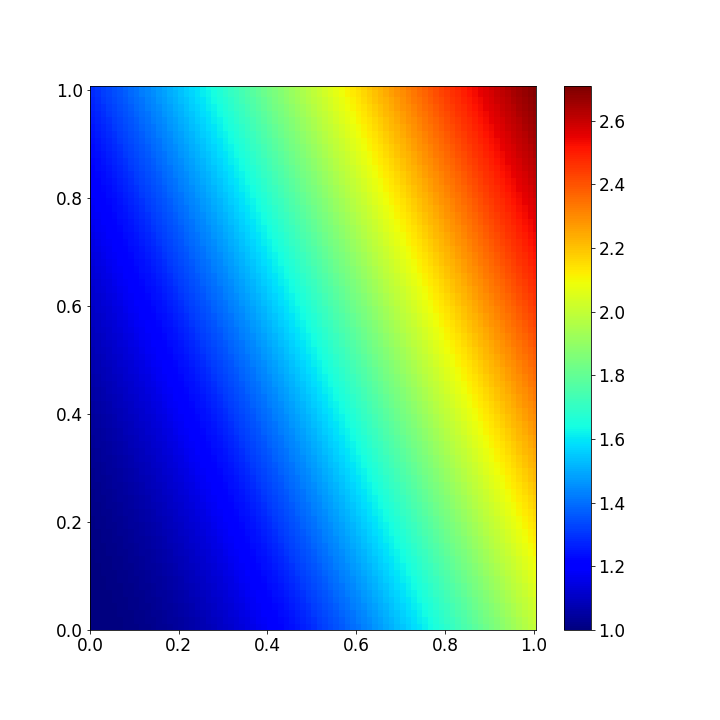
\includegraphics[width=.5\textwidth]{compare_2d_3d/field3d_80.png}
\caption{Проекция 3D решения (слева), 2D решение (справа)}
\label{fig:compare_2d_3d_fields}
\end{figure}
Визуально значения не отличаются. Построим разницу и сравним ее с ошибкой, полученной при сравнении с аналитическим решением на рис. \ref{fig:difference}:
\begin{figure}[H]
\centering
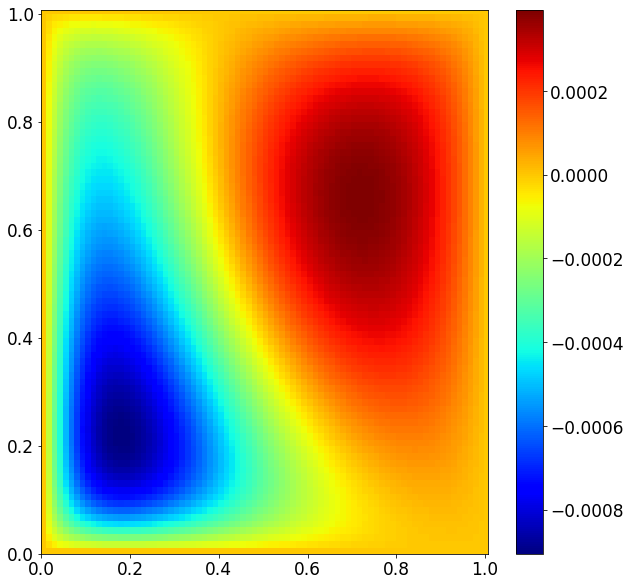
\includegraphics[width=.5\textwidth]{compare_2d_3d/difference.png}\hfill
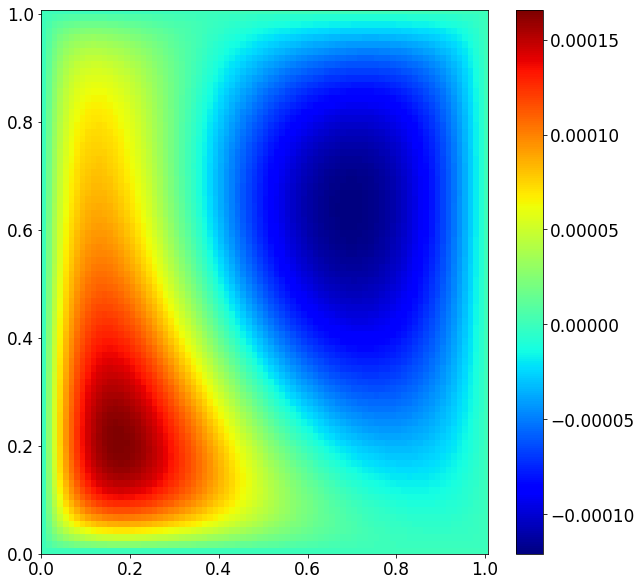
\includegraphics[width=.5\textwidth]{compare_2d_3d/error.png}
\caption{Разница между решениями 2D и 3D (слева), разница между аналитическим решением и 2D (справа)}
\label{fig:difference}
\end{figure}
По графикам видно, что разница между решениями, полученными разными методами, отражает значение реальной ошибки. Это позволяет исследовать порядок ошибки, не зная аналитического решения.

\subsubsection{Исследование сеточной сходимости неявной схемы в 3D \label{heat:convergence}}
Проведем исследование сходимости реализованного численно решения нелинейного уравнения теплопроводности в 3D с помощью методов из раздела \ref{implementation:convergence}
\paragraph{Постановка численного эксперимента}
Используем полностью неявную схему неявным методом Эйлера для аппроксимации производной по времени. Получим задачу теплопроводности из известного аналитического решения с помощью символьной математики (раздел \ref{implementation:symbolic}).
В качестве решения возьмем неотрицательную функцию:
\begin{equation}
u(x, y, z, t) = 2 + \sin \left(\pi \cdot \left( 0.5x + 0.25y + 0.75z - t\right) \right)
\end{equation}
В качестве нелинейного коэффициента возьмем:
\begin{equation}
\alpha(u) = \frac{u^2}{9}
\end{equation}

Минимальное количество точек по одной оси - 11, шаг $h$ уменьшается в 2 раза. Шаг по времени пропорционален $h^2$. Решим задачу на 4 сетках.
Выпишем вид источника, полученного с помощью символьной математики:

\begin{multline}
    \nu(x, y, z, t) = \\ - 0.0972 \pi^{2} \left(\sin{\left(\pi \left(- t + 0.5 x + 0.25 y + 0.75 z\right) \right)} + 2\right)^{2} \cdot \sin{\left(\pi \left(- t + 0.5 x + 0.25 y + 0.75 z\right) \right)} \\ + 0.194 \pi^{2} \left(\sin{\left(\pi \left(- t + 0.5 x + 0.25 y + 0.75 z\right) \right)} + 2\right) \cdot \cos^{2}{\left(\pi \left(- t + 0.5 x + 0.25 y + 0.75 z\right) \right)} \\ - \pi \cos{\left(\pi \left(- t + 0.5 x + 0.25 y + 0.75 z\right) \right)}
\end{multline}

\paragraph{Результаты расчета}
На рис. \ref{fig:heat3d_time_error} слева приведена зависимость нормы относительной $L_2$ ошибки от времени. Ошибка вычисляется как разность численного и аналитического решения во всем пространстве в конкретный момент времени. Справа зависимость нормы $L_2$ ошибки на последнем шаге расчета от шага сетки.

\begin{figure}[H]
\centering
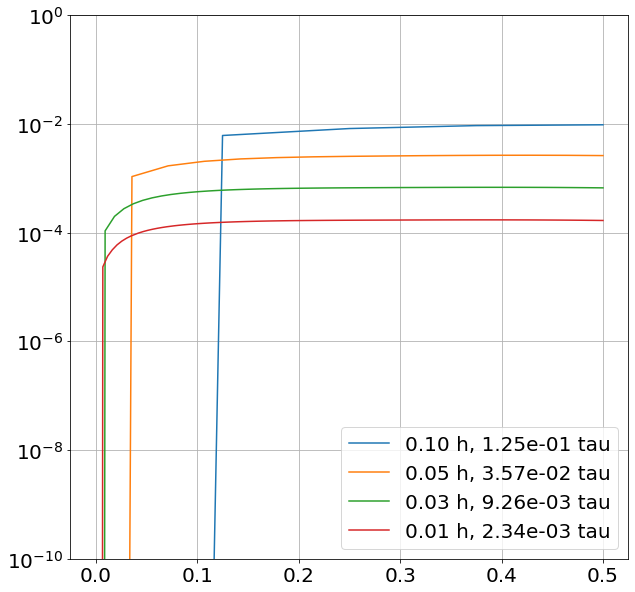
\includegraphics[width=.5\textwidth]{heat3d/time-error.png}\hfill
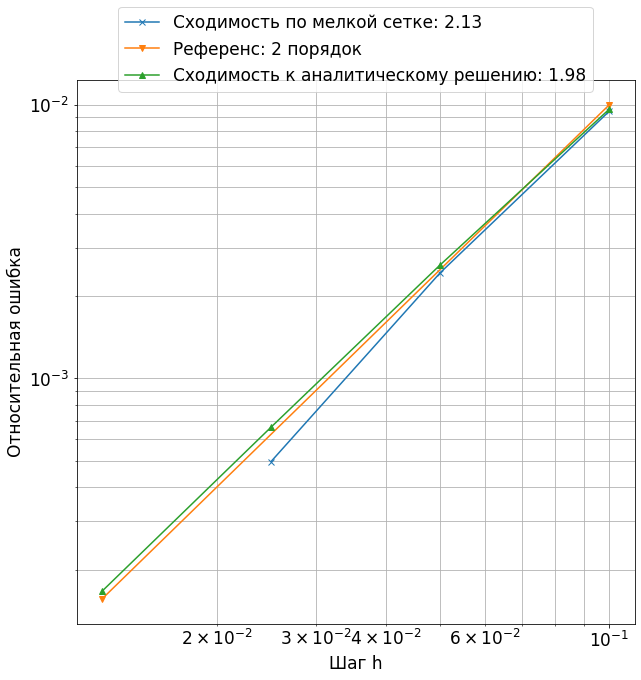
\includegraphics[width=.5\textwidth]{heat3d/convergence.png}
\caption{Зависимость нормы ошибки от времени (слева), зависимость нормы ошибки от шага сетки в последний момент расчета (справа)}
\label{fig:heat3d_time_error}
\end{figure}

Рассмотрим решения и ошибки на одной из 2D проекции расчетной области: $z = z_{max} / 2$ на рис. \ref{fig:heat3d_field}:

\begin{figure}[H]
\centering
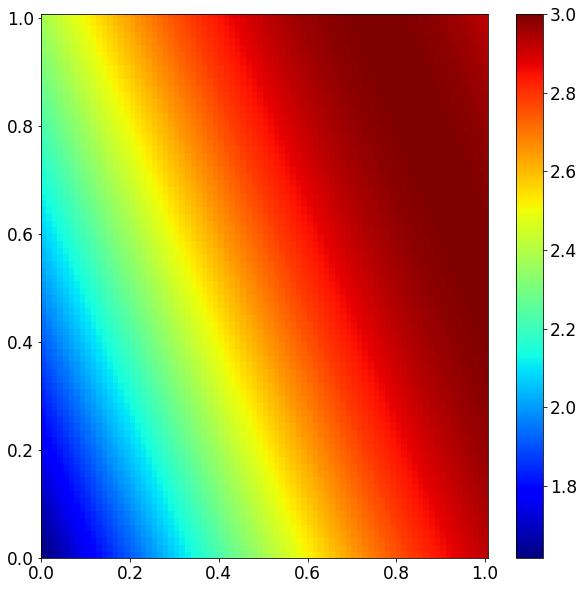
\includegraphics[height=.45\textwidth]{heat3d/solution_80dots.png}
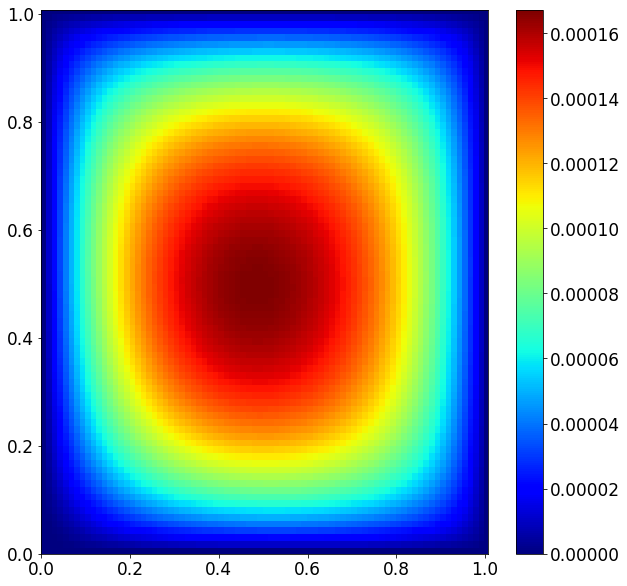
\includegraphics[height=.45\textwidth]{heat3d/rel_err_80dots.png}
\caption{Проекция $z=0.5z_{max}$: решение (слева) и относительная ошибка (справа)}
\label{fig:heat3d_field}
\end{figure}

\subsection{Вывод}
Подведем итог результатов, полученных в данной главе. Мы рассмотрели неявные по времени методы решения нелинейной задачи. В трехмерной постановке лучше всего себя зарекомендовала такая связка алгоритмов: полностью неявная схема, метод Ньютона для решения нелинейной системы, метод сопряженных градиентов для решения СЛАУ. Наиболее эффективным предобуславливателем был ILU и многосеточный метод. 

\section{Исследование системы гидродинамики на основе метода функционала плотности \label{dhd}}
\subsection{Постановка задачи}
\subsubsection{Метод функционала плотности}
Рассмотрим задачу течения 2-х несмешиваемых жидкостей в керне. Движение жидкости описывается с помощью \textit{метода функционала плотности}. Система уравнений состоит из уравнений неразрывности и уравнения движения.
Подробное описание и теоретический вывод метода функционала плотности приведен в \cite{demyanov, dhd_spe}. Остановимся на результатах его применения, которые пригодятся в данной работе.
\par
Уравнения неразрывности каждой жидкости выражены через их мольные плотности - молярные массы на единицу объема. Если сложить их, можно получить стандартный вид уравнения неразрывности. 
Задача решается в кубе $D \in \mathbb{R}^3; t \in (0, T)$. Решение ищется в виде мольных плотностей $n_i = [n_1, n_2]^T$ и вектора среднемассовой скорости $v_a$. Все функции, из которых составлены уравнения, и неизвестные решения считаются гладкими.

\begin{equation} \label{eq:dhd_system}
\begin{cases}
\frac{\partial n_{i}}{\partial t}+\frac{\partial\left(V_{b}n_{i}\right)}{\partial x_{b}}-\frac{\partial}{\partial x_{b}}\left(P_{i j}\frac{\partial\Phi_{j}}{\partial x_{b}}\right)=\vartheta_{i}^{n}(t,x_{a}) 
\\ \\
\frac {\partial\rho V_{a}} {\partial t} + \frac {\partial} {\partial x_{b}} \left( \rho V_{b}V_{a} - \tau_{ab} \right) + n_i \frac{\partial \Phi_i}{\partial x_a}=\vartheta_{a}^{M}(t,x_{a})
\end{cases}
\end{equation}
где $\rho = M_i \cdot n_i$ - плотность ($M_i$ - молярные массы), $P_{ij}$ - матрица диффузии. $\vartheta^n_i$ и $\vartheta^M_a$ - источник плотности и внешняя сила. 
\\
$\tau_{ab}$ - тензор вязкости:
\begin{equation} \label{eq:viscosity_tensor}
\tau_{ab} = (\eta - \frac{2}{3} \mu) \frac {\partial V_c} {\partial x_c} \delta_{ab} + \mu \left( \frac{\partial V_{a}}{\partial x_{b}}+\frac{\partial V_{b}}{\partial x_{a}} \right) 
\end{equation}
где $\mu$ - сдвиговая вязкость, а $\eta$ - объемная вязкость.

\subsubsection*{Обобщенная свободная энергия}
В методе функционала плотности используется термодинамический потенциал - обобщенная свободная энергия:
\begin{equation} \label{eq:helmholz_energy}
w = f + \frac{1}{2} \nu_{ij} \frac {\partial n_i} {\partial x_a} \frac {\partial n_j} {\partial x_a}
\end{equation}
где $f = f(n_i)$ - свободная энергия смеси, а $\nu_{ij} = \nu_{ij} (n_i)$ - положительно определенная матрица, определяющая поверхностное натяжение между компонентами. Смесь стремится к наиболее выгодному состоянию, в котором обобщенная свободная энергия принимает минимальное значение. Исследуемые жидкости несмешиваемые. Поэтому $f(n_i)$ определятся так, чтобы иметь минимумы в точках, полностью заполненных одной жидкостью. Такие устойчивые состояния и есть \textit{фазы} в нашей модели. Мы рассматриваем двухфазную смесь - свободная энергия принимает минимальное значение, если в точке находится только одна из двух жидкостей.
\par
В рамках данной работы используется физическая модель двух жидкостей с такой свободной энергией:
\begin{equation}
\frac{1}{f} = \frac{1}{f_0} + \frac{1}{f_1}
\end{equation}
Где $f_i$ - свободная энергия каждой жидкости, задающаяся такой формулой:
\begin{equation}
f_i = (n_i - \overline n_i)^T E_i (n_i - \overline n_i)
\end{equation}
где $\overline n_i$ - мольные плотности в чистых фазах, $E_i$ - матрицы свободной энергии. Смысл данной формулы - сделать минимальной свободную энергию в фазе.
\par
Дифференцируя $w$  из формулы \eqref{eq:helmholz_energy} по $n_i$, получим обобщенный химический потенциал $\Phi$:
\begin{equation}
\Phi_i := \frac{\partial w}{\partial n_i} =\frac{\partial f}{\partial n_{i}}+\frac{1}{2}\frac{\partial\nu_{jk}}{\partial n_{i}}\frac{\partial n_{j}}{\partial x_{a}}\frac{\partial n_{k}}{\partial x_{a}}-\frac{\partial}{\partial x_{a}}\left(\nu_{ij}\frac{\partial n_{j}}{\partial x_{a}}\right)
\end{equation}
Через него можно выразить тензор напряжений:
\begin{equation}
\sigma_{ab} = (\omega-\Phi_{j}n_{j})\delta_{ab}-\nu_{ij}\frac{\partial n_{i}}{\partial x_{a}}\frac{\partial n_{j}}{\partial x_{b}}
\end{equation}
Отсюда получим давление:
\begin{equation}
p=-\frac{1}{3}\sum_a{\sigma_{aa}}=(\Phi_{j}n_{j}-\omega)+\sum_a{\frac{\nu_{ij}}{3}\frac{\partial n_{i}}{\partial x_{a}}\frac{\partial n_{j}}{\partial x_{a}}}
\end{equation}
\subsubsection{Сферическая симметрия}
В данной работе для проведения численных экспериментов рассматривается система функционала плотности в сферических координатах с учетом сферической симметрии. Такой подход позволяет решать численно одномерную систему и получать результаты, учитывающие влияние поверхностного натяжения. Получим вид системы \eqref{eq:dhd_system} в сферических координатах. В силу сферической симметрии все функции зависят только от $r$:
\begin{equation}
\frac{\partial}{\partial \theta} = 0;
\quad
\frac{\partial}{\partial \varphi} = 0 
\end{equation}
Воспользуемся выражениями для дивергенции, градиента и оператора Лапласа в сферических координатах c учетом симметрии:
\begin{equation}
\frac{\partial f_i}{x_i} \rightarrow \frac{1}{r^2} \frac{\partial}{\partial r} ( r^2 f_i );
\quad
\frac{\partial g}{x_i} \rightarrow \frac{\partial g}{\partial r};
\quad
\frac{\partial^2 \varphi}{\partial x_i \partial x_i} \rightarrow \frac{1}{r^2} \frac{\partial}{\partial r} \left( r^2 \frac{\partial \varphi}{\partial r} \right)
\end{equation}
Исследуемая система находится на отрезке $(0, R)$ на оси $r$, все векторы коллинеарны этой оси. Получим систему функционала плотности на этой оси:
\begin{equation} \label{eq:dhd_spherical}
\begin{cases}
\frac{\partial n_{i}}{\partial t} + \frac {1} {r^2} \frac{\partial}{\partial r}\left( r^2 \left[V_{r} n_{i} - P_{i j}\frac{\partial\Phi_{j}}{\partial r} \right] \right)=\vartheta_{i}^{n}(t, r) 
\\ \\
\frac {\partial\rho V_{r}} {\partial t} + \frac {1} {r^2} \frac {\partial} {\partial r} \left[ r^2 \left( \rho V_{r}^2 - \tau_{rr} \right) \right] + n_i \frac{\partial \Phi_i}{\partial r}=\vartheta^{M}(t, r)
\end{cases}
\end{equation}
В рамках данной работы мы принимаем в \eqref{eq:helmholz_energy} $\nu_{ij} = const$. Перепишем формулы для химического потенциала и вязкости:
\begin{equation}
\Phi_i = \frac{\partial f}{\partial n_i} - \nu_{ij} \left[ \frac{1}{r^2} \frac{\partial}{\partial r} \left( r^2 \frac{\partial n_j} {\partial r} \right) \right]
\end{equation}
\begin{equation}
\tau_{rr} = (\eta - \frac{2}{3} \mu) \frac{1}{r^2} \frac{\partial \left( r^2 V_r\right) }{\partial r} + 2\mu \frac{\partial V}{\partial r}
\end{equation}
где по индексу $r$ суммирование не ведется.
Таким образом, изучается трехмерная капля одной жидкости внутри другой с учетом сферической симметрии. При этом численно решается одномерная задача.

\subsubsection{Начальные и граничные условия \label{dhd:boundary_conditions}}
\paragraph{Начальные условия}
\begin{equation} \label{eq:initial_conditions_dhd}
n_i \vert_{t=0} = n_{i, 0} (x_i); \quad V_a \vert_{t=0} = V_{a, 0}(x_i)
\end{equation}

Рассматриваются 3 вида граничных условий: \textit{условия Дирихле}, \textit{условия камня} и \textit{условия симметрии}:
\paragraph{Условия Дирихле}
\begin{equation} \label{eq:dirichlet_dhd}
n_i \vert_{\partial D} = n_{i, 0}(r); \quad \left. V_r \right \vert_{\partial D} = V_{r, 0}(r) 
\end{equation}
\paragraph{Условия камня} используются для моделирования твердой стены, через которую не может течь жидкость. В рамках сферической симметрии его можно использовать на внешней границе. Для реализации условия камня необходимо приравнять к нулю скорости на границе клеток камня, мольные концентрации внутри камня: 
\begin{equation}
n_i \vert_{\textrm{rock}} = 0;
\quad \quad
V_r \vert_{\textrm{rock}} = 0
\end{equation}
Потока через каменную границу быть не должно. Рассмотрим, из каких слагаемых состоит поток в уравнении \eqref{eq:dhd_spherical}. Все компоненты, кроме одной, приравняются к нулю сами. Диффузионный поток на границе с камнем нужно приравнять к нулю вручную:
\begin{equation}
\left. P_{ij} \cdot \frac{\partial \Phi_j}{\partial r} \right \vert_{\textrm{rock}} = 0
\end{equation}
\paragraph{Условия симметрии} используются в центре сферической симметрии. Скалярные поля должны быть симметричны относительно центра капли, а векторные --- антисимметричны. Центр находится в точке $r = 0$:
\begin{equation} \label{eq:symmetry}
\left. \left. \frac{\partial n_i (r, t)} {\partial r} \right \vert_{r=0} = 0; 
\quad \quad
V_r(r, t) \right \vert_{r=0} = 0
\end{equation}
\subsection{Дискретизация \label{dhd:discretization}}
Второй порядок аппроксимации достигается методом, описанным в главе \ref{methods:space_derivative}. Используем постоянный шаг $h$ для сеток по пространству. Введем названия для разных сеток:
\begin{itemize}
\item D-точки находятся в центрах ячеек: $\quad r^D_{i} = \left[ \frac{h}{2} + h \cdot i\right] \quad \quad i = \overline{0, M-1}$
\item U-точки находятся на гранях между ячейками: $\quad r^U_{i} = \left[ h \cdot i\right] \quad \quad i = \overline{0, M}$
\end{itemize}
Значения $n_i$ определяются в D-точках, $V_r$ --- в U-точках.
\par
Введем операторы интерполяции $I^D$, $I^U$ с одной сетки на другую. Верхний индекс указывает, с какой сетки происходит интерполяция. Аналогичным образом введем операторы производной с разных сеток: $D^{\times} \approx \frac {\partial } {\partial r}$. Здесь $\times$ - либо D, либо U. Данный оператор переносит значения на другую сетку, так как использует формулу центральной разности --- значение производной вычисляется посередине между соседними точками для повышения точности. Приведем примеры действия операторов на вектор $q^\times$ на рис. \ref{fig:dhd_points}
\begin{figure}[H]
  \centering
  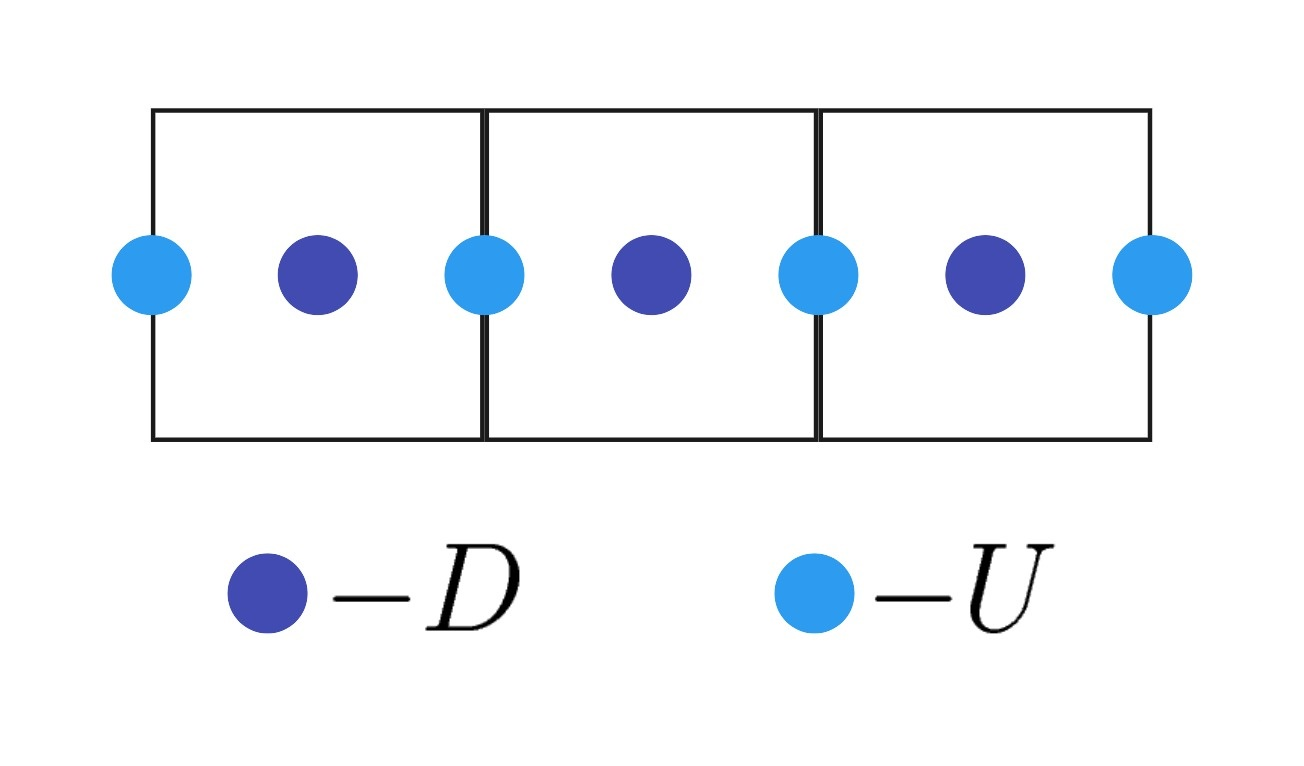
\includegraphics[valign = c, width = .5\linewidth]{common_images/dhd_points.jpg} \qquad
  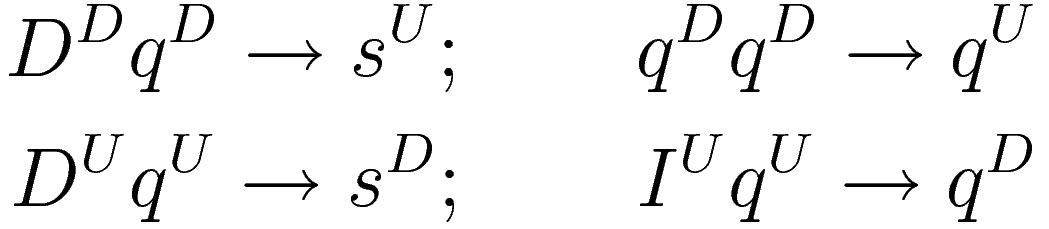
\includegraphics[width = .3\linewidth]{common_images/dhd_interpolation.png}
  \caption{Визуализация точек на разных сетках и примеры действия операторов интерполяции и дифференцирования}
  \label{fig:dhd_points}
\end{figure}

\subsubsection*{Аппроксимация граничных условий симметрии} 
Центр симметрии на левой границе (рис. \ref{fig:dhd_symmetry}). Граница расположена между соседними D-точками, чтобы аппроксимировать производную от $n_i$ по формуле центральной разности. Однако для расчета нужна крайняя U-точка, которая находится левее последней D-точки. Поэтому необходимо использовать дополнительную U-точку в $r = -h$. Значение вектора $V_r$ в ней определяется из соображений симметрии --- он должен быть направлен противоположено $V_r(h)$. Получаем дискретный вид граничных условий симметрии:
\begin{equation}
n_{i, 0} = n_{i, 1};
\quad \quad
V_{r, 0} = -V_{r, 2};
\quad \quad
V_{r, 1} = 0
\end{equation}
\begin{figure}[H]
\centering
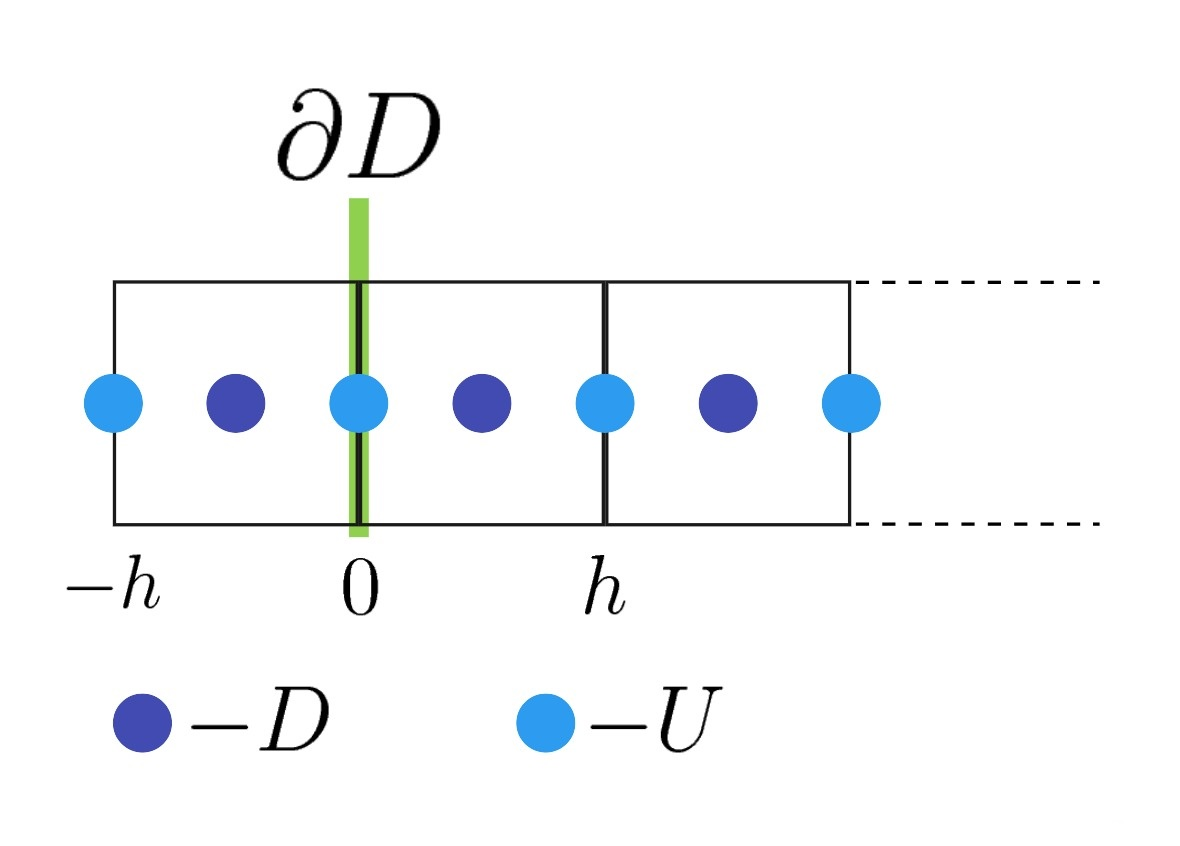
\includegraphics[width=0.5\textwidth]{common_images/symmetry.jpg}
\caption{Граничное условие симметрии. Внизу подписан тип точек.}
\label{fig:dhd_symmetry}
\end{figure}

\subsection{Особенности реализации численных схем \label{dhd:features}}
Запишем численно задачу функционала плотности \eqref{eq:dhd_system} в терминах производных на разных сетках из раздела \ref{dhd:discretization}. 
\begin{equation} \label{eq:dhd_difference}
\begin{cases}
\frac{\partial n_i}{\partial t} + \frac {1} {r^2} D^U_0 \left[ r^2 \left( V_r \cdot I^D_0 n_i - P_{ij} \cdot D^D_0 \Phi_j\right) \right] = \vartheta_{i}^{n}
\\ \\
\frac{\partial \left( \rho(I^D_0 n_i) \cdot V_r \right)}{\partial t} + \frac{1}{r^2} D^U_0 \left[ r^2 \left( \rho(n_i) \cdot I^U_0 V^2_r - \tau_{rr} \right) \right] + I^D_0 n_i \cdot D^D_0 \Phi_i = \vartheta^M
\end{cases}
\end{equation}
Для удобства функции от $n_i$ и $V_r$ определены на тех сетках, на которых они нужны в системе \eqref{eq:dhd_difference}. Покажем, как они вычисляются численно. Будем использовать верхний индекс, для уточнения сетки, например $n^D_i$ и $V_r^U$:
\begin{equation}
P_{ij}^U = P_{ij} \left( I^D_0(n_i) \right)
\end{equation}
\begin{equation}
\tau_{rr}^D = (\eta - \frac{2}{3} \mu) \frac{1}{r^2} D^U_0 \left( r^2 V_r \right) + 2 \mu D^U_0 V_r
\end{equation}
\begin{equation}
\Phi^D_i = \frac{\partial f}{\partial n} - \nu_{ij} \frac{1}{r^2} \left( r^2 \frac{\partial n_j}{\partial r} \right)
\end{equation}
Функция $\rho$ указана в системе \eqref{eq:dhd_difference} со своими аргументами в явном виде, поскольку используется на разных сетках.
\subsubsection*{Интегрирование по времени}
Аппроксимация производной по времени методами из раздела \ref{methods:time_integration} приводит либо к явному, либо к неявному методу решения. В рамках данной работы реализованы оба этих метода. Анализ устойчивости уравнения \eqref{eq:dhd_system} показывает, что шаг по времени $\tau$ существенно ограничен для явного метода. Поэтому интерес для исследования представляет решение неявным методом. 
\subsubsection*{Неявное решение}
Рассмотрим используемый алгоритм неявного решения согласно главе \ref{methods}:
\begin{itemize}
\renewcommand{\labelitemii}{•}
% \renewcommand{\labelitemiii}{•}
    \item Цикл шагов по времени 
    \begin{itemize}
        \item Цикл итераций метода Ньютона (раздел \ref{methods:newton})
        \begin{itemize}
            \item Цикл итераций метода решения линейной системы (раздел \ref{methods:linear_solvers})
            \item Перерасчет матрицы Якоби, если необходимо (раздел \ref{implementation:operator_preconditioning})
        \end{itemize}
    \end{itemize}
\end{itemize}
Матрица Якоби не обладает тридиагональным видом \eqref{mat:tridiagonal}, несмотря на то, что система одномерная. Причина в том, что вектор неизвестных в системе \eqref{eq:newtons_method_system} включает в себя как $n_i$, так и $V_r$: 
\begin{equation}
\mathbf{x} = \left[ n_0 \dots n_{0, M-1}; \quad n_1 \dots n_{1, M-1}; \quad V_{r, 0} \dots V_{r, M}\right]
\end{equation}
Здесь  $M$ - количество D-точек, $M+1$ - количество U-точек. Нелинейная система $\mathbf{F}(\mathbf{x}) = 0$ связывает $n_0$, $n_1$ и $V_r$ зависимостью. Кроме того, в системе присутствует 4-я производная. Она приводит к зависимости значений в 5 точках друг от друга. Поэтому необходимо применять общие методы решения разреженных линейных систем, рассмотренные ранее. Будем использовать  \textit{методы подпространства Крылова}. Матрица Якоби не симметрична, поэтому нам подойдут методы GMRES или BiCGStab (разделы \ref{methods:gmres}, \ref{methods:bicgstab}).
\subsubsection*{Вычисление действия матрицы Якоби}
Поскольку мы используем {методы подпространства Крылова}, мы можем вычислить матрицу Якоби в виде оператора, способного действовать на вектор. Реализованы численный и аналитический подходы, описанные в главе \ref{implementation:operator_preconditioning}.
Прямой метод используется для проверки аналитического.
Рассмотрим, как дифференцируется сложная функция $\mathbf{F}(\mathbf{x})$ для системы функционала плотности, записанной численно \eqref{eq:dhd_difference}:
\begin{equation} 
    \left\{
        \begin{multlined}
            d\frac{\partial n_i}{\partial t} + \frac {1} {r^2} D^U_0 \left[ r^2 \left( dV_r \cdot I^D_0 n_i + V_r \cdot I^D_0 dn_i - dP_{ij} \cdot D^D_0 \Phi_j - P_{ij} \cdot D^D_0 d\Phi_j\right) \right] = 0 
            \\ \\
            \shoveleft{
                d\frac{\partial \left( \rho(I^D_0 n_i) \cdot V_r \right)}{\partial t} + \frac{1}{r^2} D^U_0 \left[ r^2 \left( d\rho(n_i) \cdot I^U_0 V^2_r + \rho(n_i) \cdot I^U_0 (2V_r dV_r) - d\tau_{rr} \right) \right] +
            }
            \\
            +  I^D_0 dn_i \cdot D^D_0 \Phi_i + I^D_0 n_i \cdot D^D_0 d\Phi_i = 0
        \end{multlined}
    \right.
\end{equation}
Здесь дифференциал от $\frac{\partial}{\partial t}$ мы оставили в общем виде, поскольку его вид зависит от выбранной дискретизации. Важно, что только значения на нелинейном слое по времени считаются функциями, по которым происходит дифференцирование. Значения на известных предыдущих слоях входят в решаемую систему $\mathbf{F}(\mathbf{x}) = 0$ уже как константы. Например, для неявного метода Эйлера (раздел \ref{methods:time_integration}):
\begin{equation}
     d\frac{\partial n_i}{\partial t} = \frac{dn_i}{\tau}; 
     \quad
     d\frac{\partial \left( \rho(I^D_0 n_i) \cdot V_r \right)}{\partial t} = \frac{d\rho(I^D_0 n_i) \cdot V_r + \rho(I^D_0 n_i) \cdot dV_r}{\tau}
\end{equation}
Дифференциалы функций $\rho, P_{ij}, \Phi_i, \tau_{rr}$ рассчитываются аналогично. Покажем на примере $\rho$:
\begin{equation}
d \rho = d\left( M_i n_i \right) = M_i dn_i
\end{equation}

\subsubsection*{Особенности применения предобуславливателей}
При расчетах мы пользовались такими предобуславливателями: полный метод LU, разреженный метод ILU и многосеточный метод (разделы \ref{methods:lu}, \ref{methods:ilu}, \ref{methods:multigrid}). Полный метод не занимает слишком много времени, так как система одномерная. По сравнению с ним, разреженный метод не дает прироста производительности в одномерной задаче. Однако такой подход плохо масштабируется, поэтому мы рассмотрели многосеточный метод.
\par
Применение многосеточного метода отличается от его применения к скалярной задаче теплопроводности \eqref{eq:heat_equation}. При построении векторного оператора интерполяции на более грубую сетку необходимо учесть, что в одном векторе переменных нелинейной системы $\mathbf{x}$ содержатся значения $n_0$, $n_1$ и $V_r$. Именно этим методом планируется решать трехмерную систему функционала плотности \eqref{eq:dhd_system}, поскольку там размер матрицы будет значительно больше.

\subsubsection*{Компиляция кода}
В формуле \eqref{eq:dhd_difference} используются аналитические гладкие функции, например производная свободной энергии $\frac{\partial f}{\partial n_i}$. Согласно подходу, описанному в разделе \ref{implementation:cuda}, такие производные вычисляются аналитически с помощью символьной математики. Для использования физической модели жидкости достаточно задать вид свободной энергии. Результатом описанного подхода является сгенерированная формула на языке С с атрибутами CUDA, которая встраивается в численную схему. Покажем, как выглядит код таких формул на примере производной свободной энергии $\frac{\partial f}{\partial n_i}$ для конкретной жидкости:
\begin{lstlisting}[style=CStyle]
static __device__
void compute_chemical_potentials(double *n, double *dw) {
   dw[0] = 2.1780926979276557e-6*(-69.757105602213599*n[0] - 418.78244767971137*n[1] + 3594.1684922005115)*((n[0] - 55.555555555555557)*(16.199999999999999*n[0] - 900.
   0) + 97.255693077323699*(n[0] - 55.555555555555557)*n[1] + (97.255693077323699*n[0] - 5403.0940598513171)*n[1] + 677.58193767828004*pow(n[1], 2))*((n[1] - 8.0)*
   (781.25*n[1] - 6250.0) + 112.135530762532*(n[1] - 8.0)*n[0] + (112.135530762532*n[1] - 897.084246100256)*n[0] + 18.6785528011068*pow(n[0], 2))/pow(0.
   0014758362707047335*(n[0] - 55.555555555555557)*(16.199999999999999*n[0] - 900.0) + 0.14353347937604158*(n[0] - 55.555555555555557)*n[1] + 0.0014758362707047335*
   (97.255693077323699*n[0] - 5403.0940598513171)*n[1] + 0.0014758362707047335*(n[1] - 8.0)*(781.25*n[1] - 6250.0) + 0.16549368353407115*(n[1] - 8.0)*n[0] + 0.
   0014758362707047335*(112.135530762532*n[1] - 897.084246100256)*n[0] + 0.027566485708146914*pow(n[0], 2) + pow(n[1], 2), 2) + (32.399999999999999*n[0] + 194.
   5113861546474*n[1] - 1800.0)*((n[1] - 8.0)*(781.25*n[1] - 6250.0) + 112.135530762532*(n[1] - 8.0)*n[0] + (112.135530762532*n[1] - 897.084246100256)*n[0] + 18.
   6785528011068*pow(n[0], 2))/((n[0] - 55.555555555555557)*(16.199999999999999*n[0] - 900.0) + 97.255693077323699*(n[0] - 55.555555555555557)*n[1] + (97.
   255693077323699*n[0] - 5403.0940598513171)*n[1] + (n[1] - 8.0)*(781.25*n[1] - 6250.0) + 112.135530762532*(n[1] - 8.0)*n[0] + (112.135530762532*n[1] - 897.
   084246100256)*n[0] + 18.6785528011068*pow(n[0], 2) + 677.58193767828004*pow(n[1], 2)) + (37.357105602213601*n[0] + 224.271061525064*n[1] - 1794.168492200512)*((n
   [0] - 55.555555555555557)*(16.199999999999999*n[0] - 900.0) + 97.255693077323699*(n[0] - 55.555555555555557)*n[1] + (97.255693077323699*n[0] - 5403.0940598513171)*n
   [1] + 677.58193767828004*pow(n[1], 2))/((n[0] - 55.555555555555557)*(16.199999999999999*n[0] - 900.0) + 97.255693077323699*(n[0] - 55.555555555555557)*n[1] + (97.
   255693077323699*n[0] - 5403.0940598513171)*n[1] + (n[1] - 8.0)*(781.25*n[1] - 6250.0) + 112.135530762532*(n[1] - 8.0)*n[0] + (112.135530762532*n[1] - 897.
   084246100256)*n[0] + 18.6785528011068*pow(n[0], 2) + 677.58193767828004*pow(n[1], 2)) + ((n[1] < 0) ? (
      20.0*n[0]*pow(n[1], 2)
   )  : (0)) + ((n[0] < 0) ? (
      20.0*(pow(n[0], 2) + pow(n[1], 2))*n[0] + 20.0*pow(n[0], 3)
   ) : (0));
   dw[1] = 2.1780926979276557e-6*(-418.78244767971142*n[0] - 2917.6638753565603*n[1] + 23306.188119702638)*((n[0] - 55.555555555555557)*(16.199999999999999*n[0] - 900.
   0) + 97.255693077323699*(n[0] - 55.555555555555557)*n[1] + (97.255693077323699*n[0] - 5403.0940598513171)*n[1] + 677.58193767828004*pow(n[1], 2))*((n[1] - 8.0)*
   (781.25*n[1] - 6250.0) + 112.135530762532*(n[1] - 8.0)*n[0] + (112.135530762532*n[1] - 897.084246100256)*n[0] + 18.6785528011068*pow(n[0], 2))/pow(0.
   0014758362707047335*(n[0] - 55.555555555555557)*(16.199999999999999*n[0] - 900.0) + 0.14353347937604158*(n[0] - 55.555555555555557)*n[1] + 0.0014758362707047335*
   (97.255693077323699*n[0] - 5403.0940598513171)*n[1] + 0.0014758362707047335*(n[1] - 8.0)*(781.25*n[1] - 6250.0) + 0.16549368353407115*(n[1] - 8.0)*n[0] + 0.
   0014758362707047335*(112.135530762532*n[1] - 897.084246100256)*n[0] + 0.027566485708146914*pow(n[0], 2) + pow(n[1], 2), 2) + (194.5113861546474*n[0] + 1355.
   1638753565601*n[1] - 10806.188119702634)*((n[1] - 8.0)*(781.25*n[1] - 6250.0) + 112.135530762532*(n[1] - 8.0)*n[0] + (112.135530762532*n[1] - 897.084246100256)*n
   [0] + 18.6785528011068*pow(n[0], 2))/((n[0] - 55.555555555555557)*(16.199999999999999*n[0] - 900.0) + 97.255693077323699*(n[0] - 55.555555555555557)*n[1] + (97.
   255693077323699*n[0] - 5403.0940598513171)*n[1] + (n[1] - 8.0)*(781.25*n[1] - 6250.0) + 112.135530762532*(n[1] - 8.0)*n[0] + (112.135530762532*n[1] - 897.
   084246100256)*n[0] + 18.6785528011068*pow(n[0], 2) + 677.58193767828004*pow(n[1], 2)) + (224.271061525064*n[0] + 1562.5*n[1] - 12500.0)*((n[0] - 55.555555555555557)
   *(16.199999999999999*n[0] - 900.0) + 97.255693077323699*(n[0] - 55.555555555555557)*n[1] + (97.255693077323699*n[0] - 5403.0940598513171)*n[1] + 677.
   58193767828004*pow(n[1], 2))/((n[0] - 55.555555555555557)*(16.199999999999999*n[0] - 900.0) + 97.255693077323699*(n[0] - 55.555555555555557)*n[1] + (97.
   255693077323699*n[0] - 5403.0940598513171)*n[1] + (n[1] - 8.0)*(781.25*n[1] - 6250.0) + 112.135530762532*(n[1] - 8.0)*n[0] + (112.135530762532*n[1] - 897.
   084246100256)*n[0] + 18.6785528011068*pow(n[0], 2) + 677.58193767828004*pow(n[1], 2)) + ((n[0] < 0) ? (
      20.0*pow(n[0], 2)*n[1]
   ) : (0 )) + ((n[1] < 0) ? (20.0*(pow(n[0], 2) + pow(n[1], 2))*n[1] + 20.0*pow(n[1], 3)) : (0));
}
\end{lstlisting}
Данный пример наглядно показывает необходимость использования символьной математики. Без нее для внедрения новых физических моделей жидкостей приходилось бы каждый раз вручную вычислять огромное количество производных и писать их на низкоуровневом языке. 
\par
Может показаться необычной подстановка численных значений для конкретной модели в исходный код. Следует объяснить, что данный код генерируется для каждой новой жидкости заново автоматически, а использование численных значений в исходном коде в перспективе дает компилятору простор для оптимизаций.
\subsection{Численные эксперименты}
Для всех численных экспериментов используются одни и те же настройки жидкостей:
\begin{itemize}
\item Молярные массы: $M_0 = 18, M_1 = 100$
\item Мольные плотности: $n_0 = 55.6, n_1 = 8$
\item Матрицы свободных энергий: \begin{equation}
E_0 = \left[
\begin{array}{cc}
16.2 & 97.2556930773237 \\
		97.2556930773237 & 677.58193767828
\end{array}
\right]
\end{equation}\begin{equation}
E_1 = \left[
\begin{array}{cc}
	18.6785528011068 & 112.135530762532 \\
	112.135530762532 & 781.25
\end{array}
\right]
\end{equation}
\item Матрица поверхностного натяжения: \begin{equation} \nu_{ij} =\left[
\begin{array}{cc}
\expnumber{1.87382211559043}{-10} & 0 \\
		0 & \expnumber{1.87382211559043}{-10}
\end{array}
\right] \end{equation}
\item Сдвиговые вязкости: $\mu_i  = \left[ 0.002, 0.001 \right]$
\item Объемные вязкости: $\eta_i = \left[ 0.021, 0.042 \right]$
\end{itemize}
Вязкости смеси, используемые в формуле тензора вязкости \eqref{eq:viscosity_tensor}, вычисляются по формулам:
\begin{multline}
\mu = \left(\frac{\mu_0^{1/3} \left(\left(n_0\right)^{2} + \left(n_1 - \overline n_1\right)^{2}\right)^{0.5}}{\left(\left(n_0 - \overline n_0\right)^{2} + \left(n_1\right)^{2}\right)^{0.5} + \left(\left(n_0\right)^{2} + \left(n_1 - \overline n_1\right)^{2}\right)^{0.5}} + \right.
\\
\left. + \frac{\mu_1^{1/3} \left(\left(n_0 - \overline n_0\right)^{2} + \left(n_1\right)^{2}\right)^{0.5}}{\left(\left(n_0 - \overline n_0\right)^{2} + \left(n_1\right)^{2}\right)^{0.5} + \left(\left(n_0\right)^{2} + \left(n_1 - \overline n_1\right)^{2}\right)^{0.5}}\right)^{3}
\end{multline}

\begin{multline}
\nu = \left(\frac{\nu_0^{1/3} \left(\left(n_0\right)^{2} + \left(n_1 - \overline n_1\right)^{2}\right)^{0.5}}{\left(\left(n_0 - \overline n_0\right)^{2} + \left(n_1\right)^{2}\right)^{0.5} + \left(\left(n_0\right)^{2} + \left(n_1 - \overline n_1\right)^{2}\right)^{0.5}} + \right.
\\
\left. + \frac{\nu_1^{1/3} \left(\left(n_0 - \overline n_0\right)^{2} + \left(n_1\right)^{2}\right)^{0.5}}{\left(\left(n_0 - \overline n_0\right)^{2} + \left(n_1\right)^{2}\right)^{0.5} + \left(\left(n_0\right)^{2} + \left(n_1 - \overline n_1\right)^{2}\right)^{0.5}}\right)^{3}
\end{multline}
\par
Матрица диффузии составляется таким образом, чтобы при диффузии не происходило переноса массы. За перенос массы отвечает среднемассовая скорость $V_r$. В данной работе используется формула:

\begin{equation}
    D_{ij} = \frac{5.0 \cdot 10^{-7}}{M^2_0} \cdot \left[\begin{matrix} M_1^{2} & - M_1 M_0\\- M_1 M_0 & M_0^2 \end{matrix}\right]
\end{equation}
В экспериментах использовались такие численные алгоритмы:
\begin{itemize}
\item Интегрирование по времени неявным методом 2 порядка по 3 точкам (раздел \ref{methods:back-diff})
\item Метод Ньютона решения нелинейной системы (раздел \ref{methods:newton})
\item Алгоритм GMRES решения СЛАУ (раздел \ref{methods:gmres})
\item Предобуславливатель LU (раздел \ref{methods:lu})
\item Действие матрицы Якобы вычислялось аналитическим методом, значения матрицы не хранились (раздел \ref{methods:computing_jacobi})
\end{itemize}

\paragraph{Выбор шага по времени и пространству} Во всех экспериментах, кроме исследования сеточной сходимости, шаг по времени $\tau$ выбирался таким образом. Задавался начальный шаг по времени $\tau_0$. С каждым шагом $\tau$ увеличивался на 10\%. Так $\tau$ доходил до такого значения, когда метод Ньютона не сходился. Тогда $\tau$ уменьшался на 10\%, пока методу Ньютона не удавалось сойтись. Стандартный шаг по пространству $h = \expnumber{2.4}{-6}$.

\subsubsection{Автоматическое тестирование}
Перечислим методы автоматического тестирования из раздела \ref{implementation:testing}, которые реализованы в данной задаче:
\begin{itemize}
\item Тестируются операторы производной
\item Решение неявным методом сравнивается с явным решением
\item Проверяется закон сохранения массы в задачах без источников
\end{itemize}
Закон сохранения массы проверялся с учетом сферических координат по формуле:
\begin{equation}
m = \int_{D} \rho(\mathbf{x}) d\mathbf{x} = \int_0^\pi \sin(\theta) d\theta \int_0^{2\pi} d\varphi \int_0^R r^2 \rho(r) dr \approx 4\pi h \sum_{i=0}^{M-1} r_i^2 \rho_i
\end{equation}

\subsubsection{Распад \label{dhd:interface}}
Исследуемые жидкости несмешиваемые. Поэтому при любых начальных условиях, если в задаче нет источников, мы ожидаем увидеть одно и то же стационарное решение --- смесь из двух жидкостей распадется на отдельные фазы. 
\par
Возьмем граничные условия (раздел \ref{dhd:boundary_conditions}): \textit{симметрия} слева и \textit{камень} справа. Заполним расчетную область равномерной смесью двух жидкостей. Разобьем расчетную область на 100 точек.
Сначала жидкость разваливается на капли, а затем образуется стабильная граница между двумя жидкостями. Рассмотрим, как эволюционирует такая система на рис. \ref{fig:decay}.
\begin{figure}[H]
\centering
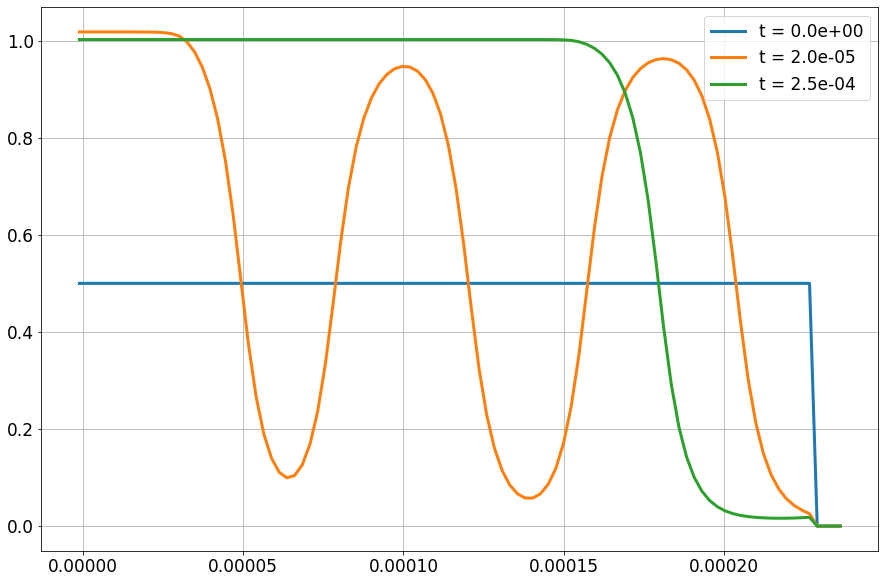
\includegraphics[width=.7\textwidth]{dhd_decay/decay.png}
\caption{Установление интерфейса между жидкостями. Показано процентное содержание первой жидкости в разные моменты времени.}
\label{fig:decay}
\end{figure}
\subsubsection{Кросс-валидация}
Реализованная программа численного решения системы функционала плотности \eqref{eq:dhd_spherical} сравнивается с результатами симулятора \textit{DHD 3D}, описанного в публикации \cite{dhd_spe}. Данная программа реализует физическую модель, описываемую системой функционала плотности \eqref{eq:dhd_system}. Перечислим особенности численной схемы \textit{DHD 3D}:
\begin{itemize}
\item Явный метод
\item Декартова система координат
\item 3D область пространства
\item Шаг по пространству $h = \expnumber{2.4}{-6}$
\item Шаг по времени $\tau = \expnumber{1}{-10}$
\end{itemize}
\paragraph{Постановка эксперимента}
Стационарное распределение мольных плотностей берется из эксперимента \ref{dhd:interface}. Делается линейная интерполяция в 3D сферу. Далее производится расчет \textit{DHD 3D}, используя эту сферу как начальное условие. Так как программы реализуют одну и ту же физическую модель, интерфейс не должен измениться.
\par
На рис. \ref{fig:cross_validation_vals} отложены значения относительной мольной плотности первой жидкости по оси, исходящей из центра капли. Значения нормированы на мольную плотность в чистой фазе. На графике показывается процентное содержание первой жидкости в зависимости от $r$. Черным цветом обозначено стационарное распределение, полученное в данной работе неявным методом. Другими цветами обозначены немного изменившиеся распределения после 3D расчета. Синим цветом обозначены значения, взятые по оси $x$, а желтым - лежащие под углом $45^\circ$ к оси $x$ в плоскости $xy$. 
\begin{figure}[h]
\centering
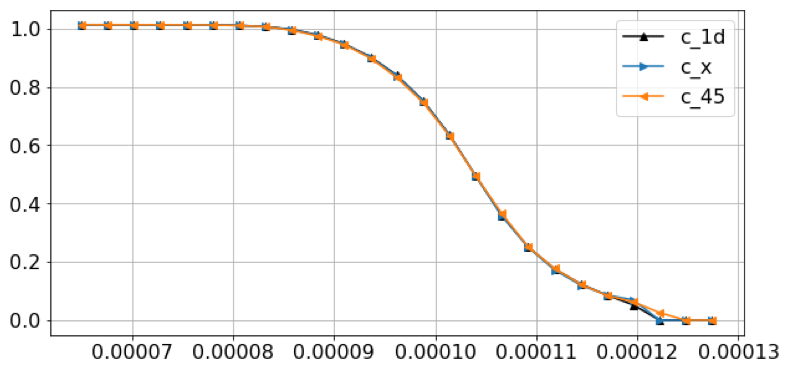
\includegraphics[scale=0.8]{dhd_cross_validation/cross_validation_vals.png}
\caption{Результаты расчета в 3d по разным осям и одномерный интерфейс}
\label{fig:cross_validation_vals}
\end{figure}
\par
Разница между этими значениями и исходным одномерным распределением показана на рис. \ref{fig:cross_validation_error}.
\begin{figure}[h]
\centering
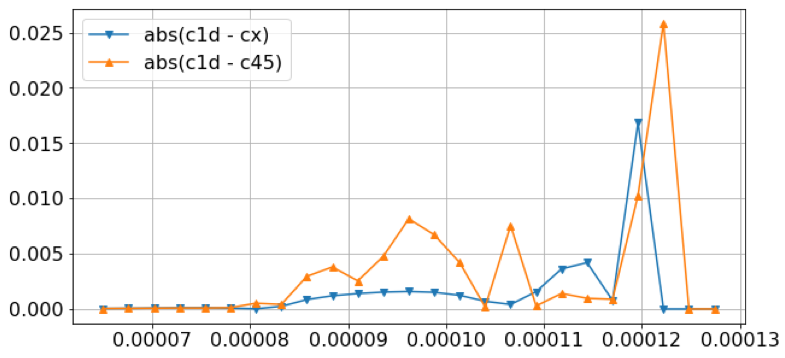
\includegraphics[scale=0.8]{dhd_cross_validation/cross_validation_error.png}
\caption{Ошибки по разным осям}
\label{fig:cross_validation_error}
\end{figure}
Основная ошибка образуется у границы. Это связано с дискретизацией границ сферы на регулярной сетке. На графике видно, что ошибка по оси $45^\circ$ больше, чем по оси $x$. Из этого делаем вывод, что основная ошибка связана с интерполяцией сферических координат в 3D.

\subsubsection{Исследование сеточной сходимости \label{dhd:convergence}}
\paragraph{Постановка эксперимента}
Проведем исследование сходимости неявной симуляции, воссоздав задачу из известного решения. Построим аналитическое решение из таких соображений. Есть некоторое распределение масс, которое перемещается из центра со скоростью $V_r(r)$:
\begin{equation}
V_r(r) = \frac{R} {10 T}  \left(1 + \operatorname{erf} \left[\frac{20} {R} \left( r - \frac{1}{2} R \right)  \right] \right)
\end{equation}
Для построения распределения масс используется функция $S(r, t)$:
\begin{equation}
S(r, t) = \left(\frac{1}{2} + \frac{1}{2} \operatorname{erf} \left[ \frac{20}{R} \left( r - t \cdot V_r(r) - {\frac{1}{2}R} \right) \right] \right)
\end{equation}
Из которой строятся поля мольных плотностей:
\begin{equation}
\begin{cases}
n_0 = \overline{n_0} \cdot S(r, t) 
\\
n_1 = \overline{n_1} \cdot (1 - S(r, t))
\end{cases}
\end{equation}
где $R = r_{max}$ и $T = t_{max}$, $\operatorname{erf}$ - интеграл распределения Гаусса (функция ошибок), $\overline{n_i}$ - мольные плотности в чистых фазах. Численные коэффициенты в формулах выбраны так, чтобы функции имели вид, показанный на рис. \ref{fig:dhd_convergence_analytic}. 
\begin{figure}[H]
\centering
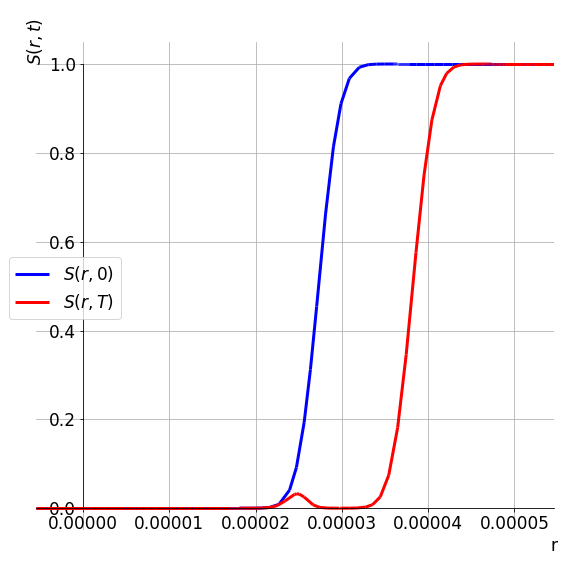
\includegraphics[width=.4\textwidth]{dhd_convergence/analytic_n.png}
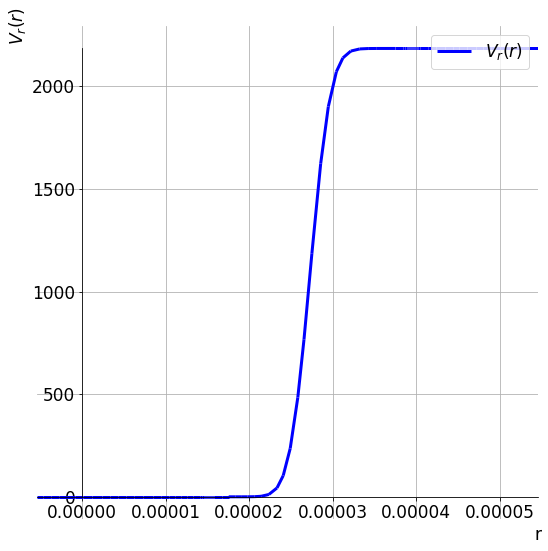
\includegraphics[width=.4\textwidth]{dhd_convergence/analytic_V.png}
\caption{Слева: функция $S(r, t)$ в моменты времени $0$  и $T$ . Справа: функция $V_r(r)$}
\label{fig:dhd_convergence_analytic}
\end{figure}
Задача решается с граничными условиями симметрии слева и камня справа. Аналитические функции решения удовлетворяют условиям симметрии \eqref{eq:symmetry}. Для аппроксимации производной по времени используется метод второго порядка по трем точкам, приведенный в разделе \ref{methods:time_integration}. Поэтому $\tau$ делится пропорционально $h$. Минимальное количество точек D сетки - 20. Задача данного эксперимента - убедиться в асимптотических свойствах сходимости схемы. Поэтому шаг по времени берется достаточно мелким.
\paragraph{Вид источника}
Правые части в уравнении \eqref{eq:dhd_difference} имеют сложный вид и вычисляются с помощью символьной математики. Мы не приводим их здесь, поскольку они заняли бы несколько листов. Приведем графики источников массы и изменения импульса на рис. \ref{fig:dhd_convergence_source}.
\begin{figure}[H]
\centering
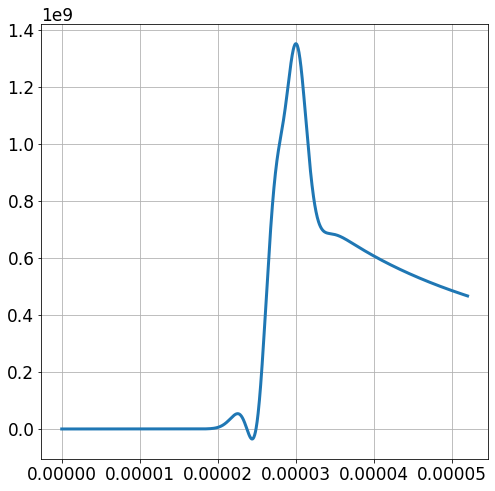
\includegraphics[width=.4\textwidth]{dhd_convergence/source_n.png}
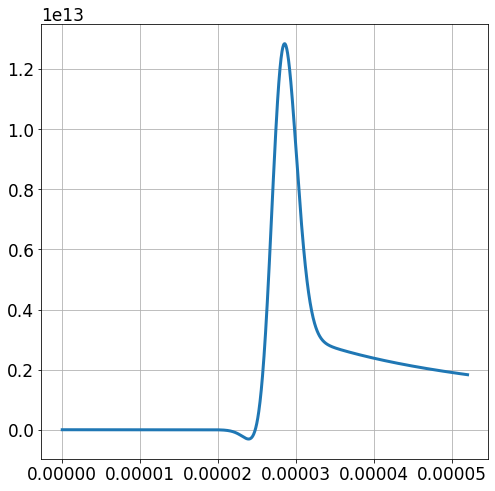
\includegraphics[width=.4\textwidth]{dhd_convergence/source_v.png}
\caption{Источники массы (слева) и изменения импульса (справа) в момент времени $t=T$.}
\label{fig:dhd_convergence_source}
\end{figure}
\paragraph{Результаты}
Результаты исследования приведены на рисунках \ref{fig:dhd_convergence_n0}, \ref{fig:dhd_convergence_n1}, \ref{fig:dhd_convergence_v} для переменных $n_0$, $n_1$ и $V_r$. Рисунки имеют одинаковую структуру. Слева изображен график нормы ошибки в зависимости от шага $h$, справа - зависимость нормы ошибки от времени. Везде используется норма $L_2$ по всему пространству в один момент времени.
\begin{figure}[H]
\centering
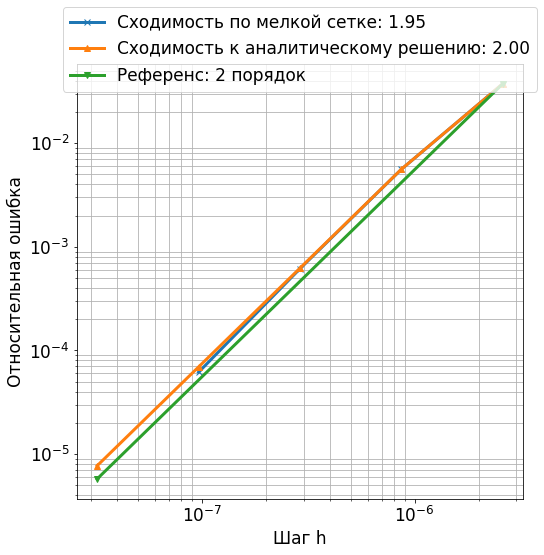
\includegraphics[width=.5\textwidth]{dhd_convergence/convergence_n0.png}\hfill
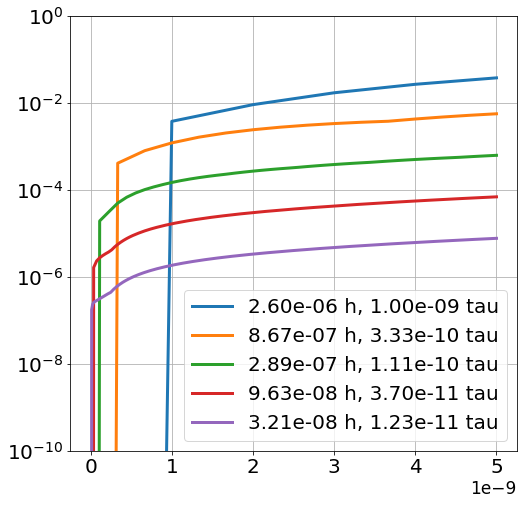
\includegraphics[width=.5\textwidth]{dhd_convergence/time_error_n0.png}
\caption{Слева: зависимость нормы ошибки от сетки при $t = T$ для $n_0$. Справа: зависимость ошибки от времени для $n_0$.}
\label{fig:dhd_convergence_n0}
\end{figure}

\begin{figure}[H]
\centering
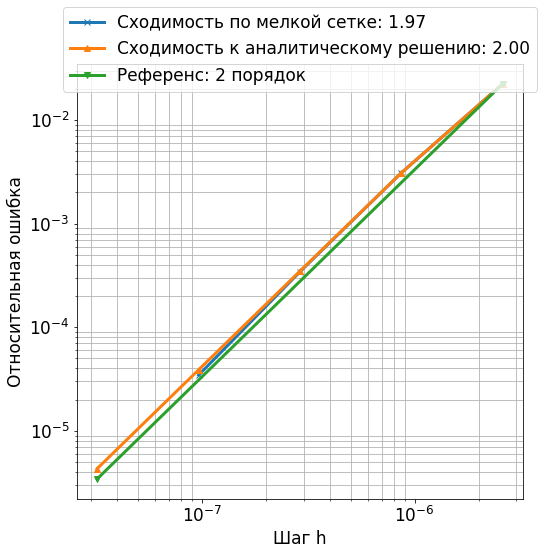
\includegraphics[width=.5\textwidth]{dhd_convergence/convergence_n1.png}\hfill
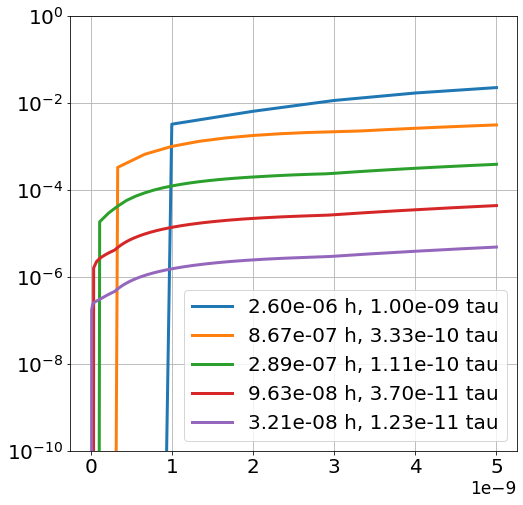
\includegraphics[width=.5\textwidth]{dhd_convergence/time_error_n1.png}
\caption{Слева: зависимость нормы ошибки от сетки при $t = T$ для $n_1$. Справа: зависимость ошибки от времени для $n_1$.}
\label{fig:dhd_convergence_n1}
\end{figure}

\begin{figure}[H]
\centering
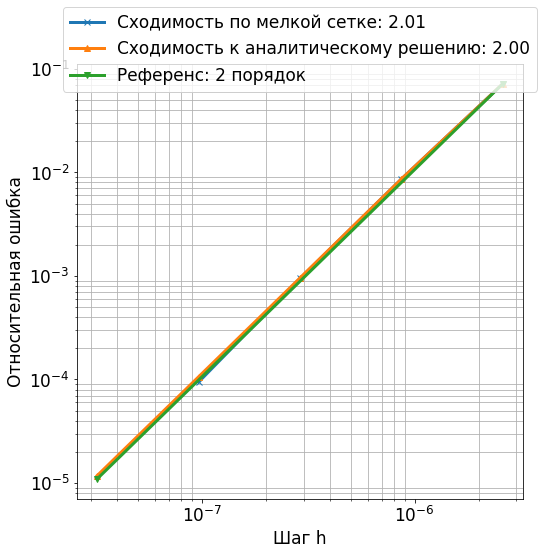
\includegraphics[width=.5\textwidth]{dhd_convergence/convergence_v.png}\hfill
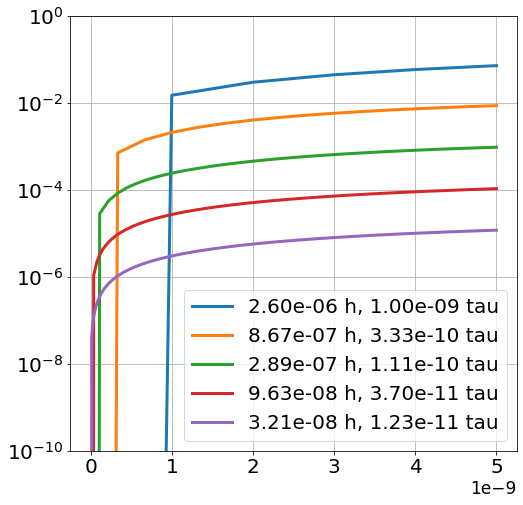
\includegraphics[width=.5\textwidth]{dhd_convergence/time_error_v.png}
\caption{Слева: зависимость нормы ошибки от сетки при $t = T$ для $V_r$. Справа: зависимость ошибки от времени для $V_r$.}
\label{fig:dhd_convergence_v}
\end{figure}

На рис. \ref{fig:dhd_convergence_error} приведена ошибка в последний момент времени для самой точной сетки. Значения нормированы на мольную плотность в чистой фазе.
\begin{figure}[H]
\centering
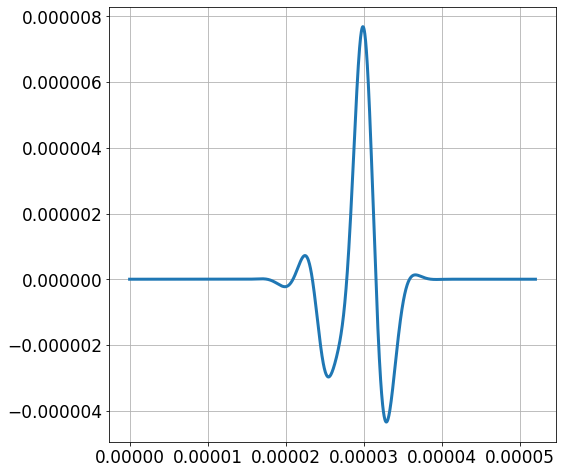
\includegraphics[width=.5\textwidth]{dhd_convergence/rel_err_n0.png}\hfill
\caption{Слева: зависимость нормы ошибки от сетки при $t = T$ для $n_0$. Справа: зависимость ошибки от времени для $n_0$.}
\label{fig:dhd_convergence_error}
\end{figure}
\subsubsection{Сравнение шага по времени неявной схемы при разных скоростях \label{dhd:t_tau}}
Для явной схемы шаг по времени ограничен условием устойчивости независимо от скорости процессов в системе. Для неявной схемы нет такого ограничения, однако при слишком большом шаге $\tau$ метод Ньютона может не сойтись. Поэтому шаг по времени все еще ограничен, хоть и на несколько порядков слабее. Это ограничение зависит от скорости процессов преобладающих в системе.
\par
Цель данного эксперимента - измерить, с каким максимальным шагом $\tau$ может идти расчет по неявной схеме. Моделируются течения с разными скоростями в области со сферической симметрией.

\subsubsection*{Постановка эксперимента} 
Капля первой жидкости расположена в центре. Ее окружает вторая жидкость. На внешней границе области расположен источник, который закачивает вторую жидкость с постоянной интенсивностью. В центре находится труба, которая поддерживает постоянную концентрацию первой жидкости, убирая излишек. Вторая жидкость вытесняет первую, и граница между двумя жидкостями постепенно приближается к центру симметрии.
\begin{figure}[H]
\centering
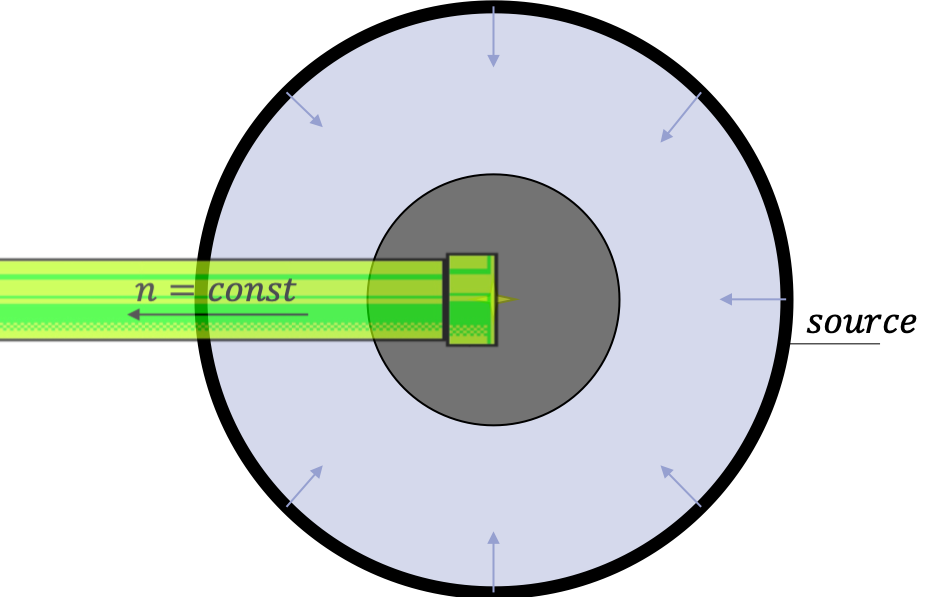
\includegraphics[width=0.5\textwidth]{dhd_t_tau/tube_experiment.png}
\caption{Постановка эксперимента.}
\end{figure}
С точки зрения численной схемы, постановка выглядит так:
\begin{itemize}
\item Граничные условия: \textit{Дирихле} слева и \textit{камень} справа
\item Начальное условие --- стационарное распределение из эксперимента \ref{dhd:interface}
\item Точечный источник массы на правой границе с постоянной интенсивностью, меняющейся от эксперимента к эксперименту
\end{itemize}

\subsubsection*{Результаты}
На рис. \ref{fig:t_tau} снизу приведена зависимость максимальной скорости в задаче от времени симуляции. Это скорость движения границы между жидкостями. Скорость пропорциональна интенсивности источника. На верхнем графике \ref{fig:t_tau} зависимость $\tau$ от времени симуляции. Шаг $\tau$ измеряется в секундах.
Расчет начинается с маленького шага, который плавно повышается, если методу Ньютона удалось сойтись. Так мы выходим на планку, показывающую максимальный шаг при данной скорости процесса. Для смеси жидкостей с используемыми параметрами шаг явной схемы, при котором симуляция остается устойчивой, $\tau_{\textrm{explicit}} \sim 10^{-9}$ с.
\begin{figure}[H]
\centering
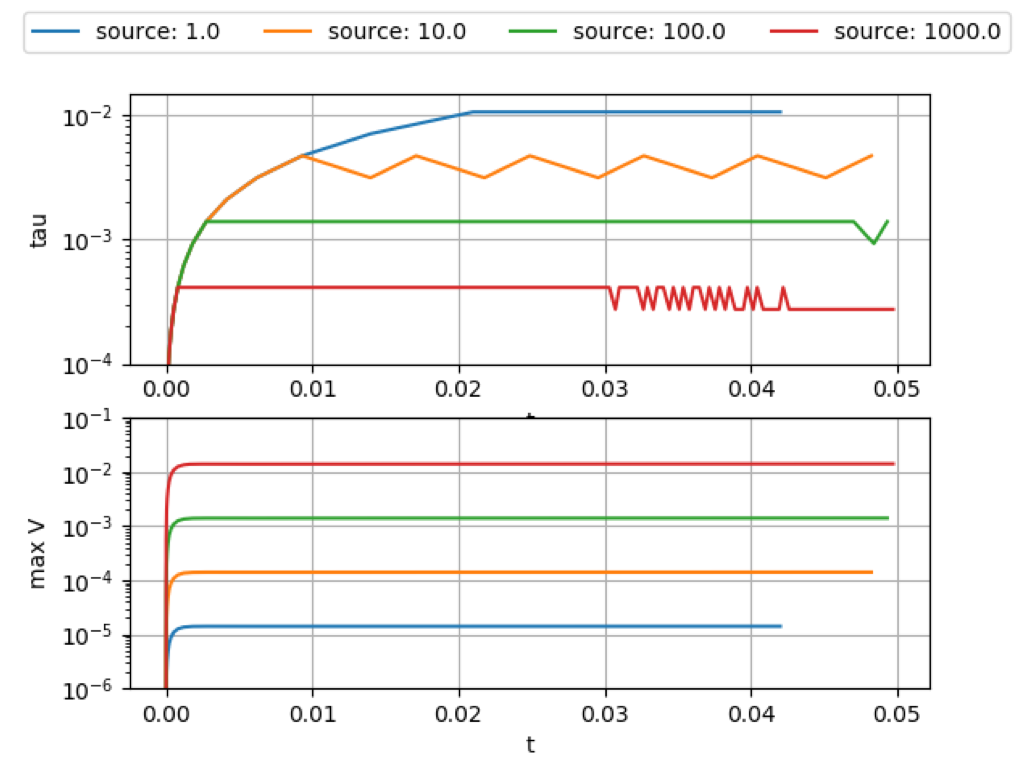
\includegraphics[width=0.8\textwidth]{dhd_t_tau/t_tau.png}
\caption{Зависимость $\tau$ от времени симуляции при различных скоростях}
\label{fig:t_tau}
\end{figure}
Полученный результат подтверждает гипотезу о зависимости шага симуляции по времени $\tau$ от скорости процессов в системе. Это значит, что использование неявной схемы будет наиболее эффективно в течениях двух жидкостей, где преобладает процесс переноса массы.
\par
Даже с достаточно большой среднемассовой скоростью шаг по времени на 5 порядков превосходит шаг для явной схемы. Нужно отметить, что при сильной диффузии ограничение шага по времени будет существеннее.  Во многих практических задачах большую часть симуляции перенос массы преобладает над диффузионными процессами. Именно в эти моменты неявная схема будет максимально эффективна.


\section{Выводы}
В данной работе мы рассмотрели подходы к реализации неявного численного метода решения системы функционала плотности. Все изученные методы сначала были реализованы на упрощенной задаче со схожей структурой --- нелинейном уравнении теплопроводности. Реализованы различные численные схемы, решающие уравнение теплопроводности. Используются одномерная, двумерная и трехмерная постановки задачи. 
\par
Предложена архитектура программы, позволяющая быстро внедрять новые физические модели и исследовать их без необходимости писать программный код. В основе данного подхода использование библиотек символьной математики и генерация нужных формул из уравнений, задаваемых физической моделью. При этом не уменьшается производительность расчета, так как генерируемые формулы встраиваются в код и компилируются. Данный подход реализован для трехмерного уравнения теплопроводности.
\par
Разработка и анализ программы для решения уравнения теплопроводности позволили выделить предпочтительные методы для реализации численного решения системы функционала плотности.
\par
На основе выбранных численных методов и архитектурных решений реализована одномерная неявная численная схема расчета системы функционала плотности. Система переведена в сферические координаты и решается со сферической симметрией. Используются автоматические тесты, проверяющие корректность изменений в программе. Проведено сравнение с другой программой, реализующей ту же самую физическую модель жидкости. Исследована сеточная сходимость.
\par
Проведен численный эксперимент, измеряющий зависимость шага по времени от среднемассовой скорости в неявной схеме системы функционала плотности. На основании данного эксперимента можно сделать следующий вывод.
Шаг по времени неявной схемы может быть на несколько порядков выше, чем шаг по времени явной схемы. При этом чем меньше максимальная среднемассовая скорость в системе, тем больше можно сделать шаг по времени. Эффективное применение неявной схемы возможно для таких течений, где медленный процесс переноса массы преобладает над процессами диффузии.
\par
В дальнейшем мы ставим себе цель реализовать трехмерную реализацию системы функционала плотности по неявному методу в поровом пространстве с использованием выбранных в данной работе численных методов и архитектурных решений.

\newpage
\bibliography{bibliography.bib}
\end{document}